In this chapter, we analyze the impact of using different participant selection and scoring algorithms on a Blockchain-based Federated Learning (BFS) system with horizontal data partition. In addition, for each scoring algorithm, we analyze how they behave and how the system is impacted by different number of clients, as well as privacy degrees. Due to the high number of plots, the communication and computation costs plots are placed at the end of the chapter.

\section{Participant Selection Algorithms}

In this set of experiments, all properties of the system are fixed, except for the participant selection algorithm, which can be either random selection or first-come first-served.

Both algorithms choose the number of clients in the same way, via a uniform random distribution. However, the clients themselves are chosen differently. Consequently, it is possible that the distribution of chosen clients is slightly different, which may affect the system performance. \autoref{fig:participations_client} illustrates client participation (represented by the bars), as well as the average number of participation per client (represented by the lines). It is clear from the plot that the distributions are different.

\begin{figure}[!ht]
    \centering
    \centering
    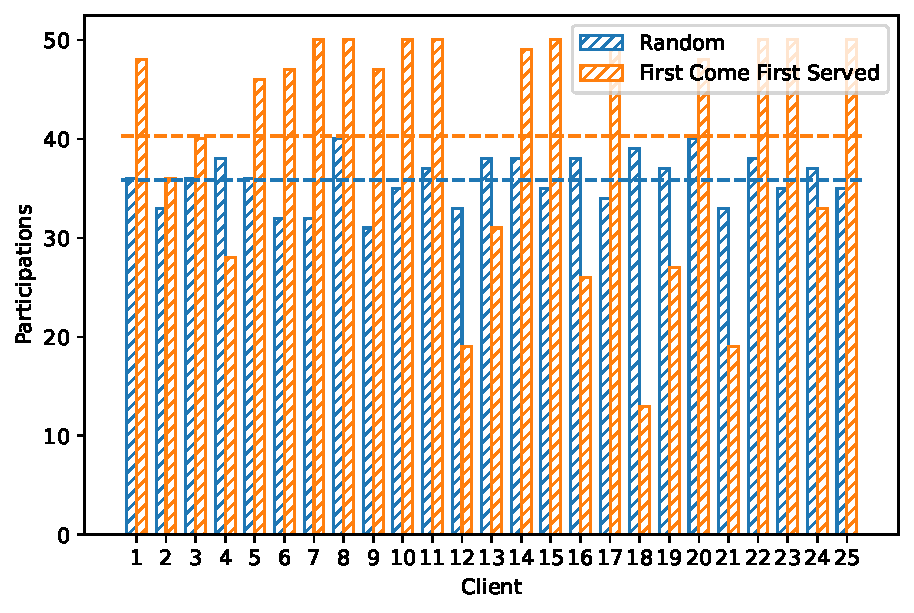
\includegraphics[width=0.7\textwidth]{graphics/selection/clients.pdf}
    \caption{Participation of Each Client Per Selection Algorithm}
    \label{fig:participations_client}
\end{figure}

On one hand, random selection presents a more uniform distribution, where each client was selected a similar number of times. On the other hand, first-come first-served presents a more skewed distribution, where some clients, such as client 1, participate many times and others, such as client 12, participate very few times. To support this observation, we calculated the standard deviation. For the random selection, the standard deviation is approximately 2.49, while for the first-come first-served it is 11.84.

From this observations, we can conclude that, by letting clients take initiative to join a round, similarly to what happens in first-come first-served, it is possible that some will end up participating more than others. By participating more often, the clients will have more influence on the global model, which can lead to skewed results.

\subsection{Execution Time, Transaction Cost, and Transaction Latency}

Regarding execution time, it can be seen from  \autoref{tab:metrics_selection} that both algorithms only differ in approximately $1.2$ minutes, which translates to a difference of $1.1$ seconds per round. In addition, the random participation was slightly faster than the first-come first-served. This negligible difference is likely caused by the fact that, in random selection, less clients participated on average per round, as shown in \autoref{fig:participations_client}. With slightly less clients, we expect that a round takes slightly less time.

\begin{table}[!ht]
\begin{tabular}{c|c|c} \hline \hline
                              & First Come First Served & Random \\ \hline \hline
E2E Time (m)                   & 19.70                   & 18.93  \\ \hline
Mean Round Time (s)            & 23.62                   & 22.70  \\ \hline
% Median Round Time (s)          & 22.06                   & 21.90  \\ \hline
Mean Transaction Latency (s)   & 1.560                   & 1.549  \\ \hline
% Median Transaction Latency (s) & 1.561                   & 1.549  \\ \hline
Mean Transaction Cost (Gas)    & 189179                  & 183124 \\ \hline
% Median Transaction Cost (Gas)  & 223471                  & 185198 \\ \hline
\end{tabular}
\caption{Execution Time, Transaction Cost, and Transaction Latency Per Participant Selection Algorithm}
\label{tab:metrics_selection}
\end{table}

\subsection{Model Accuracy and Convergence}

As it can be seen from \autoref{fig:accuracy_selection}, even though both algorithms reached identical model accuracy values at the last round, the random selection was more stable during the initial 20 rounds. This can be explained by the fact that the distribution of clients participating in each round with the random selection was closer to a uniform selection. Since the data is \textit{non-iid}, by having the same clients participate repeatedly, the model can become skewed towards their data. However, after 20 rounds, the majority of the clients had the opportunity to participate in the model, which explains why it became more and more stable.

\begin{figure}[!ht]
    \centering
    \centering
    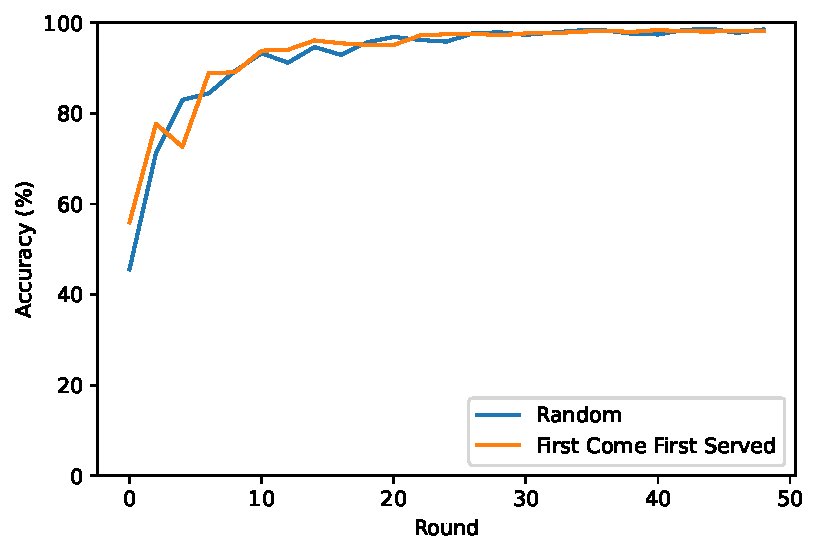
\includegraphics[width=0.7\textwidth]{graphics/selection/accuracy.pdf}
    \caption{Model Accuracy Per Participant Selection Algorithm}
    \label{fig:accuracy_selection}
\end{figure}

\subsection{Communication Costs}

\autoref{fig:net_selection} illustrates the network traffic per round for client, servers, and the blockchain processes. This algorithms solely influences which and how many clients are selected per round. Therefore, the individual communication traffic of each process is not expected to change significantly as long as the number of participants per round does not change significantly. In these experiments, we observe form \autoref{fig:participations_client} that the difference of clients participating per round is smaller than $5$. This small difference explains why the inbound traffic at the server process is slightly higher, since the server has to download weights from a higher number of clients in order to perform the aggregation.

\begin{figure}[!hpt]
    \centering
    \centering
    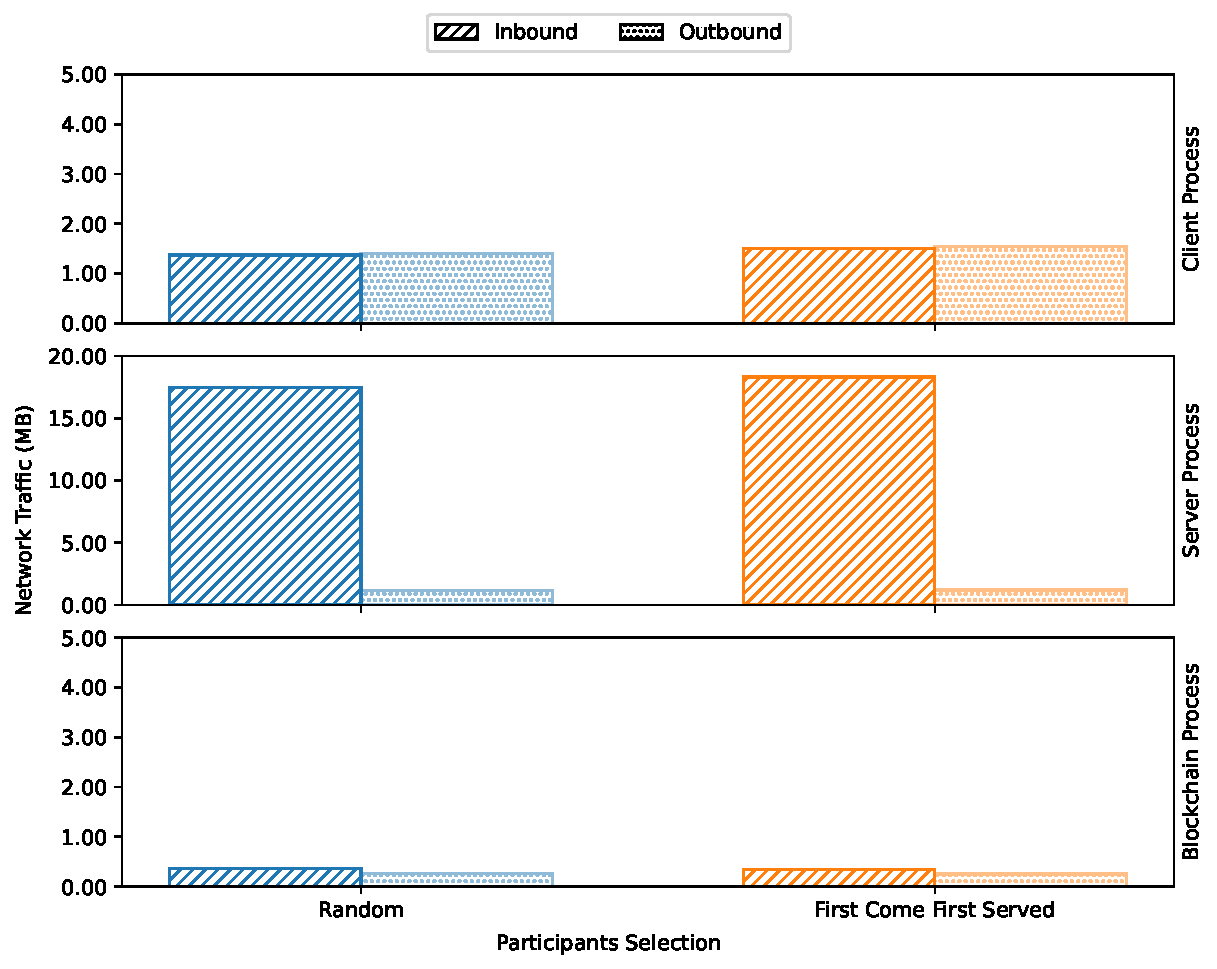
\includegraphics[width=0.8\textwidth]{graphics/selection/net.pdf}
    \caption{Network Traffic Per Round Per Participant Selection Algorithm}
    \label{fig:net_selection}
\end{figure}

\subsection{Computation Costs}

\autoref{fig:ram_selection} and \autoref{fig:cpu_selection} show the RAM usage and CPU usage per each process, respectively. Similarly to what was observed regarding the communication costs, the RAM usage at the server is slightly higher, which is explained by the additional weights to perform the aggregation. One may note that this difference happens due to the randomness of the process. In other runs, it is possible that the number of selected devices would be lower and therefore the difference would be smaller.

\begin{figure}[!hpb]
    \centering
    \centering
    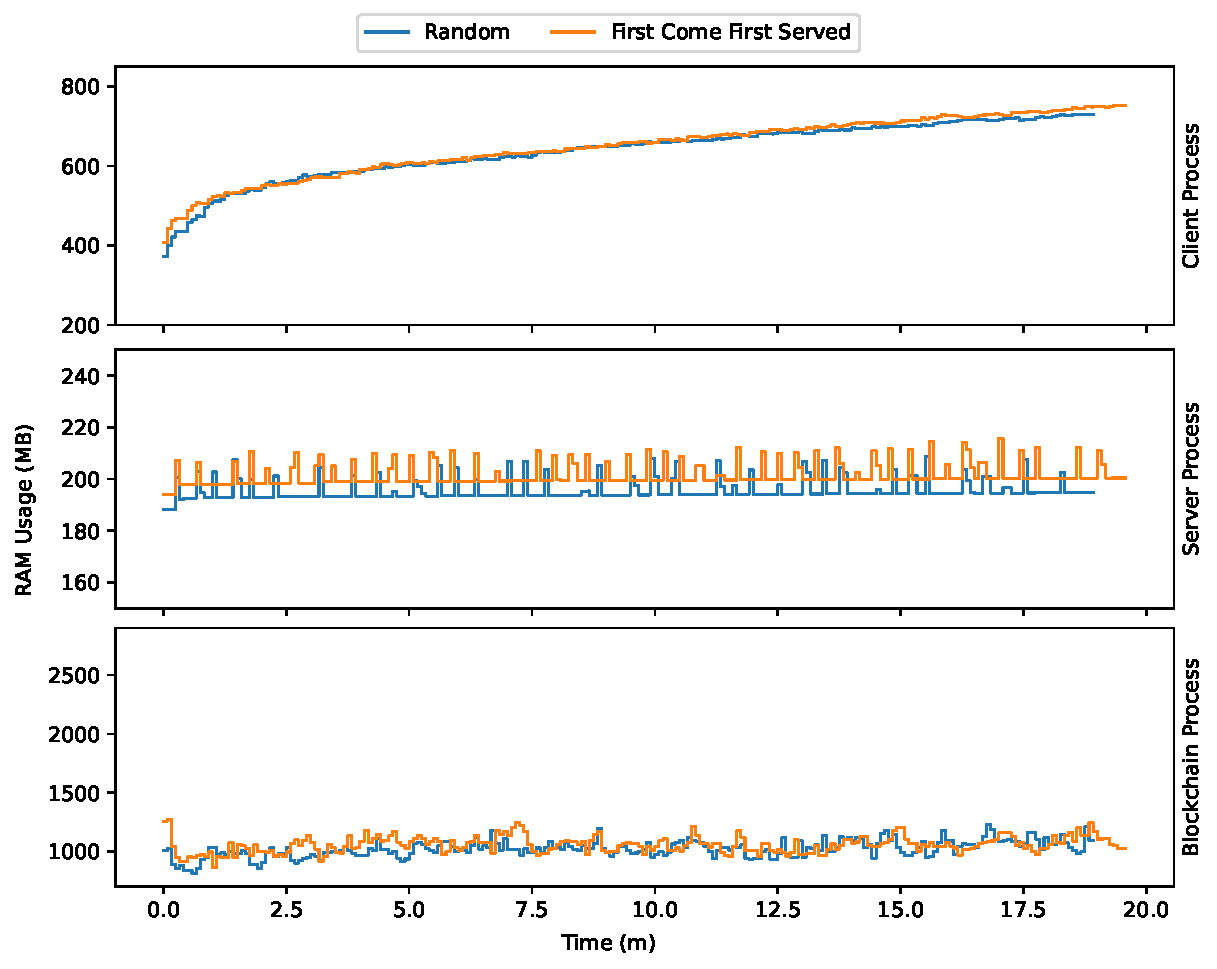
\includegraphics[width=0.8\textwidth]{graphics/selection/ram.pdf}
    \caption{RAM Usage Per Participant Selection Algorithm}
    \label{fig:ram_selection}
\end{figure}

\begin{figure}[!h]
    \centering
    \centering
    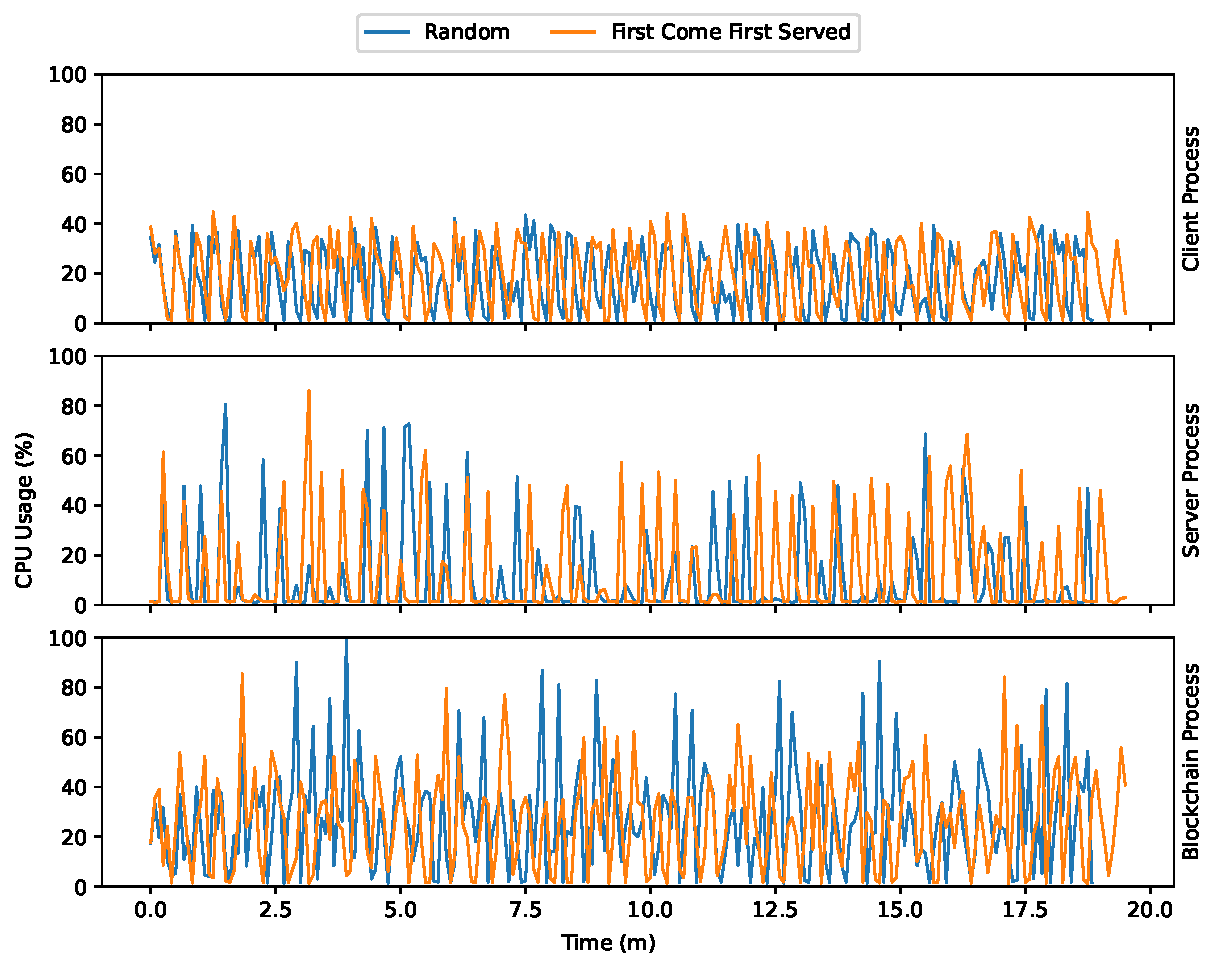
\includegraphics[width=0.8\textwidth]{graphics/selection/cpu.pdf}
    \caption{CPU Usage Per Participant Selection Algorithm}
    \label{fig:cpu_selection}
\end{figure}

\subsection{Conclusions}

From this set of experiments, we conclude that random selection performs better in terms of fairness of selection, that is, every client is given an equal chance of participating during the training process. In systems with \textit{non-iid} data, it is important to give all clients a chance to participate such that the model is trained with the most diverse data in order to produce the best results. Use of the random selection can ensure that the most amount of data is seen from most clients.

\section{Scoring Algorithms}

In this set of experiments, all properties of the system are fixed, except for the scoring algorithm, which varies between BlockFlow, Marginal Gain, Multi-KRUM, or no scoring algorithm. Then, we analyze the impact of using different numbers of clients, as well as different privacy degrees.

\subsection{Overall Comparison}\label{horizontal:scoring_overall}

We first compare the impact of the different scoring algorithms on the overall system without varying the number of clients or the privacy degree. This will let us draw some initial conclusions about the different scoring algorithms that may help explain differences observed in the remaining experiments.

\subsubsection{Execution Time, Transaction Cost, and Transaction Latency}

As it can be seen from \autoref{tab:metrics_scoring}, every scoring algorithm has different execution time and transaction cost. Firstly, one may notice that not using a scoring algorithm provides the fastest execution time as well as the lowest transaction cost. Both of these observations are explained by the fact that scoring algorithms require more transactions to submit the scores. Overall, the fastest scoring algorithm is Multi-KRUM, taking around $31$ seconds per round, while both BlockFlow and Marginal Gain are the slowest, taking both around $49$ seconds per round.

\begin{table}[!ht]
\centering
\begin{tabular}{c|c|c|c|c} \hline \hline
                               & None   & BlockFlow & Marginal Gain & Multi-KRUM \\ \hline \hline
E2E Time (m)                   & 18.93  & 40.95     & 41.38         & 26.25      \\ \hline
Mean Round Time (s)            & 22.70  & 49.11     & 49.64         & 31.48      \\ \hline
% Median Round Time (s)          & 21.90  & 49.49     & 43.97         & 31.26      \\ \hline
Mean Transaction Latency (s)   & 1.549  & 1.564     & 1.577         & 1.573      \\ \hline
% Median Transaction Latency (s) & 1.549  & 1.558     & 1.564         & 1.551      \\ \hline
Mean Transaction Cost (Gas)    & 183124 & 339645    & 257686        & 280733     \\ \hline
% Median Transaction Cost (Gas)  & 185198 & 189092    & 188994        & 187152     \\ \hline
\end{tabular}
\caption{Execution Time, Transaction Cost, and Transaction Latency Per Scoring Algorithm}
\label{tab:metrics_scoring}
\end{table}

Secondly, we observe that BlockFlow and Marginal Gain not only take the longest, but also have similar execution times. As explained in \Cref{background:scoring}, BlockFlow and Marginal Gain scores are computed by the clients, whereas Multi-KRUM scores are computed by the servers. Since the number of clients is higher than the servers, which are fixed, there are more devices performing scoring computations with BlockFlow and Marginal Gain. With more devices submitting scores, there are more transactions being submitted to the blockchain, leading to higher execution times. Therefore, it is expected that algorithms that run on the clients, such as BlockFlow and Marginal Gain, take longer than algorithms that run on the servers, such as Multi-KRUM.

Thirdly, we observe that the transaction latency is not influenced by the scoring algorithms. As it can be seen form \Cref{chapter:analysis:consensus_algorithms}, the transaction latency is mostly affected by the blockchain consensus algorithms, which, in these experiments, is fixed. In contrary, the transaction costs vary per scoring algorithm. Scoring algorithms that have more devices involved, such as scoring algorihtms executed by the servers, namely BlockFlow and Marginal Gain, have higher transaction costs. Since transaction costs work on a "supply and demand" basis, it is expected that the more transactions are required, the higher the cost will be.

\subsubsection{Model Accuracy and Convergence}

\begin{figure}[!ht]
    \centering
    \centering
    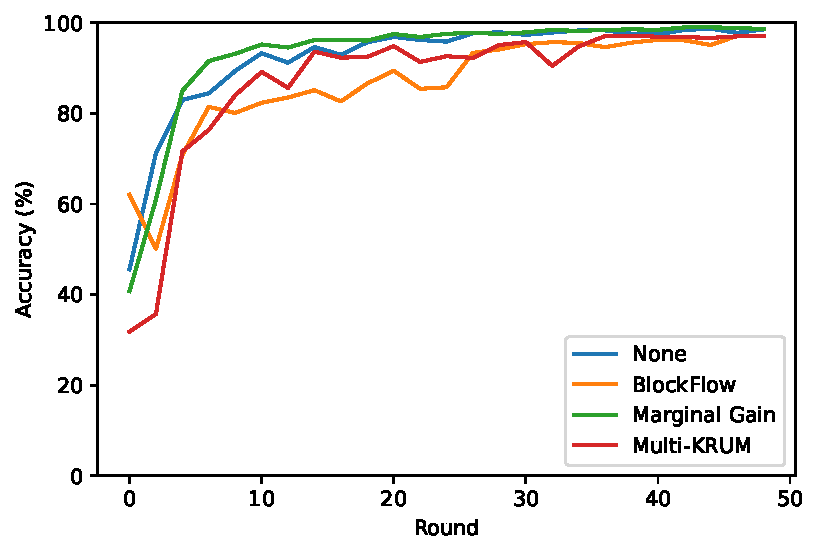
\includegraphics[width=0.7\textwidth]{graphics/scoring/accuracy.pdf}
    \caption{Model Accuracy Per Scoring Algorithm}
    \label{fig:accuracy_scoring}
\end{figure}

As it can be seen from \autoref{fig:accuracy_scoring}, all scoring algorithms reached a high model accuracy of at least  $97\%$. However, some algorithms reached higher accuracy values faster than others, that is, some converge faster. Overall, Marginal Gain converges the fastest, followed by no scoring, then by Multi-KRUM and lastly by BlockFlow.

The BlockFlow, is not only the slowest converging scoring algorithm, but also the only algorithm that does not reject submissions when aggregating, as explained in \Cref{background:scoring}. By not rejecting submissions, but still giving them a score to be used during the weighted aggregation, worse submissions are always included in the global model, which can lead to lower convergence rates. 

The Marginal Gain and Multi-KRUM algorithms both reject the worst submissions in each round and only consider the best. While the Marginal Gain uses its own score for the aggregation, the Multi-KRUM uses the number of samples of each submission, similar to the case when no scoring algorithm is used. For this reason, the Multi-KRUM algorithm convergence resembles the one of no scoring algorithm, while the Marginal Gain has a smoothest convergence curve.

\subsubsection{Communication Costs}

Communication costs also vary massively depending on which  scoring algorithm is used. Some place more strain on the clients, where others place more strain on the servers. \autoref{fig:net_scoring} presents the network traffic per round per scoring algorithm on the clients, servers, and blockchain processes.

\begin{figure}[!ht]
    \centering
    \centering
    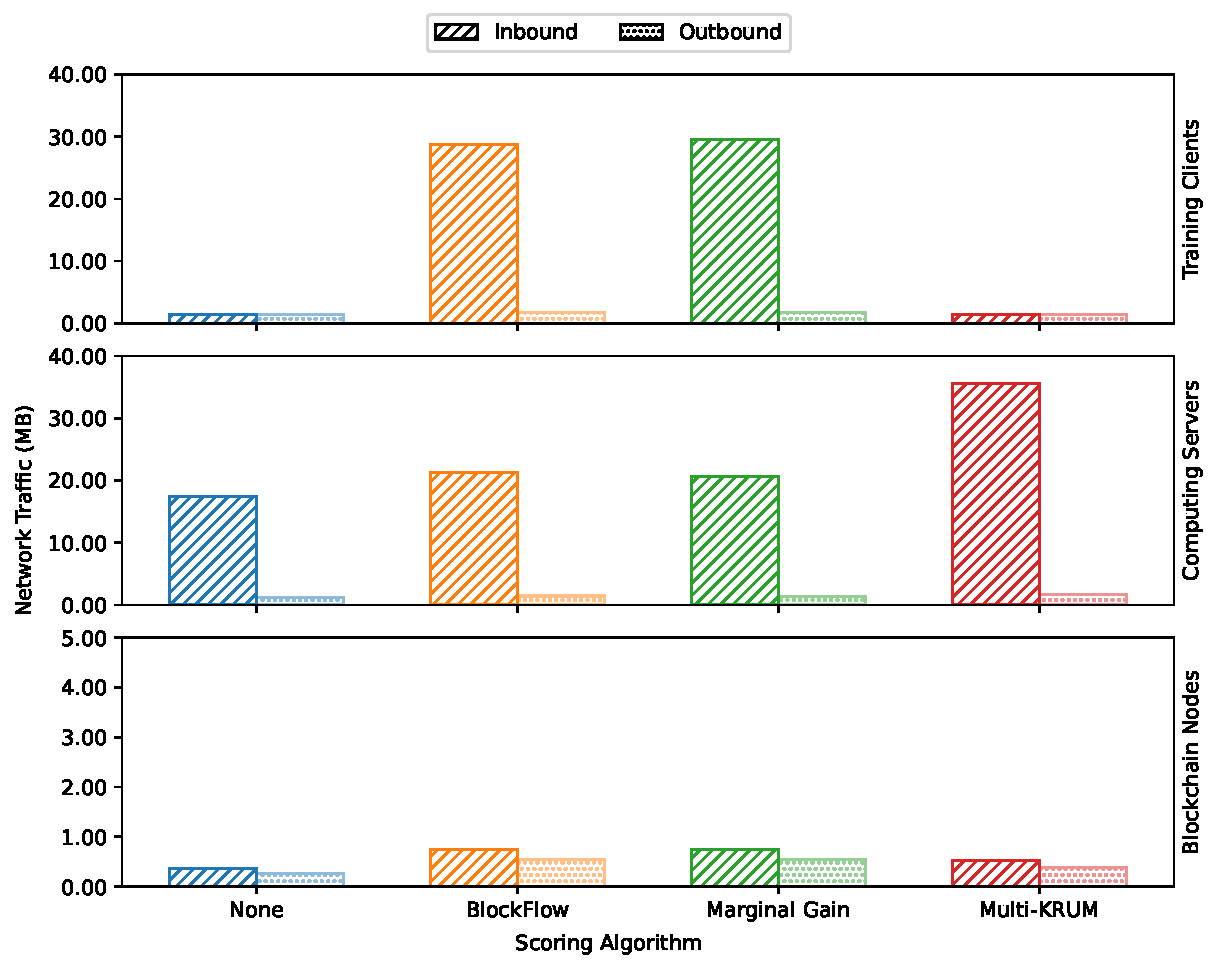
\includegraphics[width=0.8\textwidth]{graphics/scoring/net.pdf}
    \caption{Network Traffic Per Round Per Scoring Algorithm}
    \label{fig:net_scoring}
\end{figure}

Regarding the clients, there is a large difference in terms of the network traffic when comparing no scoring algorithm and the Multi-KRUM with the BlockFlow and Marginal Gain. On the one hand, the Multi-KRUM has similar traffic requirements to using no scoring algorithm on the clients because the scoring algorithm is executed on the servers. On the other hand, the BlockFlow and Marginal Gain have higher inbound traffic at the clients, while the outbound traffic remains similar. This can be explained by the fact that both BlockFlow and Marginal Gain algorithms are executed by the clients. Consequently, each client has to download the weights from all other clients in each round in order to calculate the score, leading to a higher inbound traffic.

Regarding the servers, there is not much difference between algorithms, except for the Multi-KRUM, which calculates the scores on the server. Therefore, the server downloads the weights of each client and requires additional time to calculate the scores, compared to the remaining algorithms that only download the weights once for the aggregation.

Finally, regarding the blockchain, we observe that when using the BlockFlow and Marginal Gain algorithms that there is a higher network traffic. The Multi-KRUM also requires more traffic than no scoring algorithm, but not as much as the BlockFlow or Marginal Gain. Since the number of clients is higher than the number of servers, there are more transactions when the scoring algorithm runs on the clients. When there are more transactions per round, there is more activity in the blockchain, leading to more network traffic per round.

\subsubsection{Computation Costs}

The computation costs across the servers and clients follow a similar trend to what we have seen with the communication costs. \autoref{fig:ram_scoring} and \autoref{fig:cpu_scoring} show the RAM and CPU usages on the client, server and blockchain processes, respectively.

Regarding the clients, all algorithms require similar amounts of RAM. The algorithms that run on the client, i.e., the Marginal Gain and BlockFlow, consume slightly more RAM, due to having more weights stored in memory, but the difference is negligible when compared to the total amount of RAM they consume. This can be explained by the fact that the weights are relatively small ($\approx 2$ MB) compared to the total RAM necessary to train a model. With respect to the CPU usage, it can be seen that the algorithms that run on the client, i.e., BlockFlow and Marginal Gain, have the lowest CPU idle time on the clients, while taking longer to be executed. This shows that calculating the scores on the client implies consistently higher CPU usage on the clients for longer periods of time.

Regarding the servers, it is clear that Multi-KRUM, being the only scoring algorithm that runs on the server, requires higher amount of RAM. However, the difference ($\approx 15$ MB) is not significant when considering that the servers have large amount of resources at their disposal. In addition, the Multi-KRUM also shows higher level of CPU usage, with frequent spikes to $100\%$.

Finally, regarding the blockchain, the difference of CPU and RAM usages among the different scoring algorithms is negligible. Even though the blockchain receives more transactions in total, it does not reflect on the RAM and CPU usage. The blockchain, by itself, already produces blocks at a constant rate. Therefore, the number of transactions required for the BFL system does not change significantly the CPU or RAM usage.

\begin{figure}[!hpt]
    \centering
    \centering
    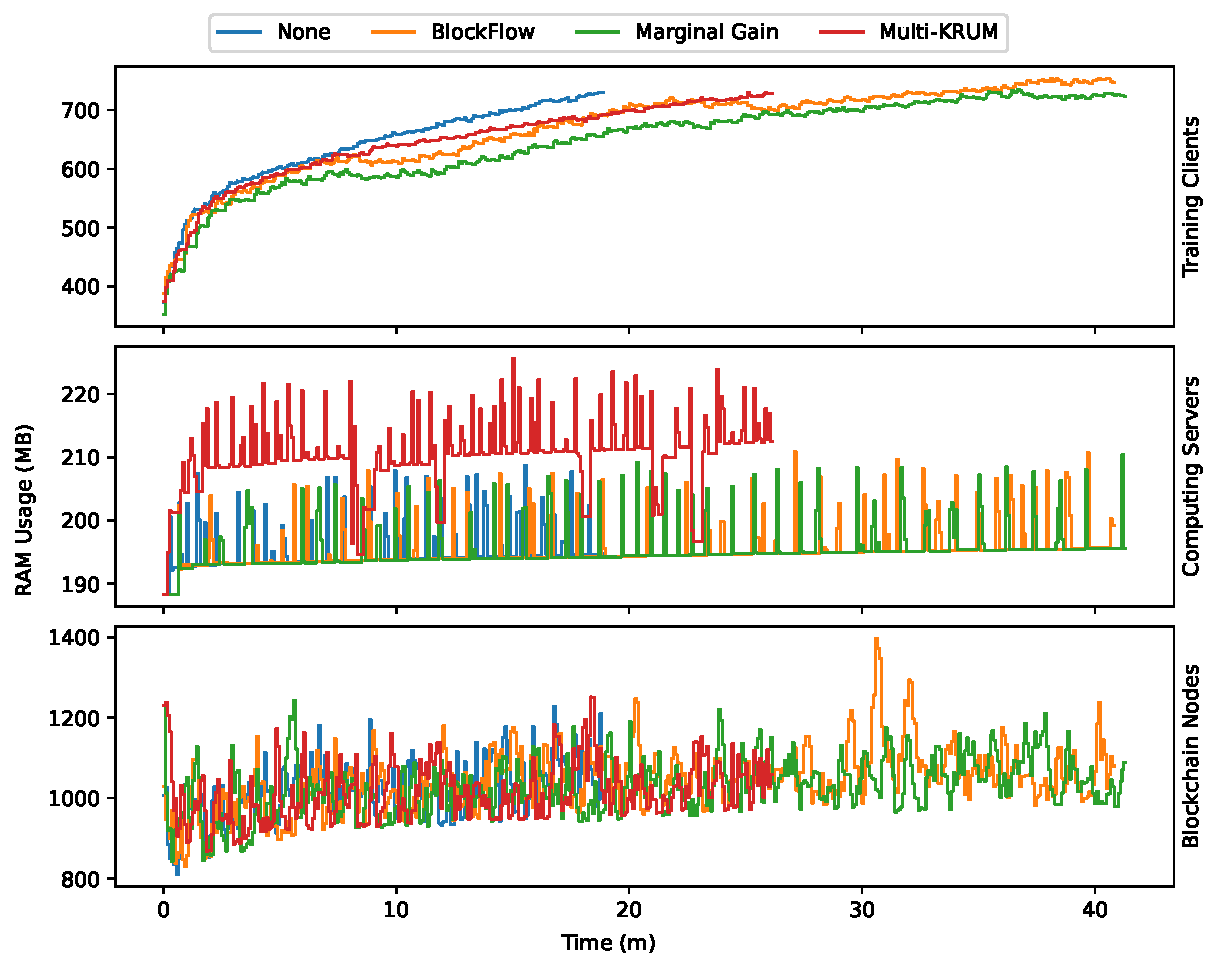
\includegraphics[width=0.8\textwidth]{graphics/scoring/ram.pdf}
    \caption{RAM Usage Per Scoring Algorithm}
    \label{fig:ram_scoring}
\end{figure}

\begin{figure}[!hpb]
    \centering
    \centering
    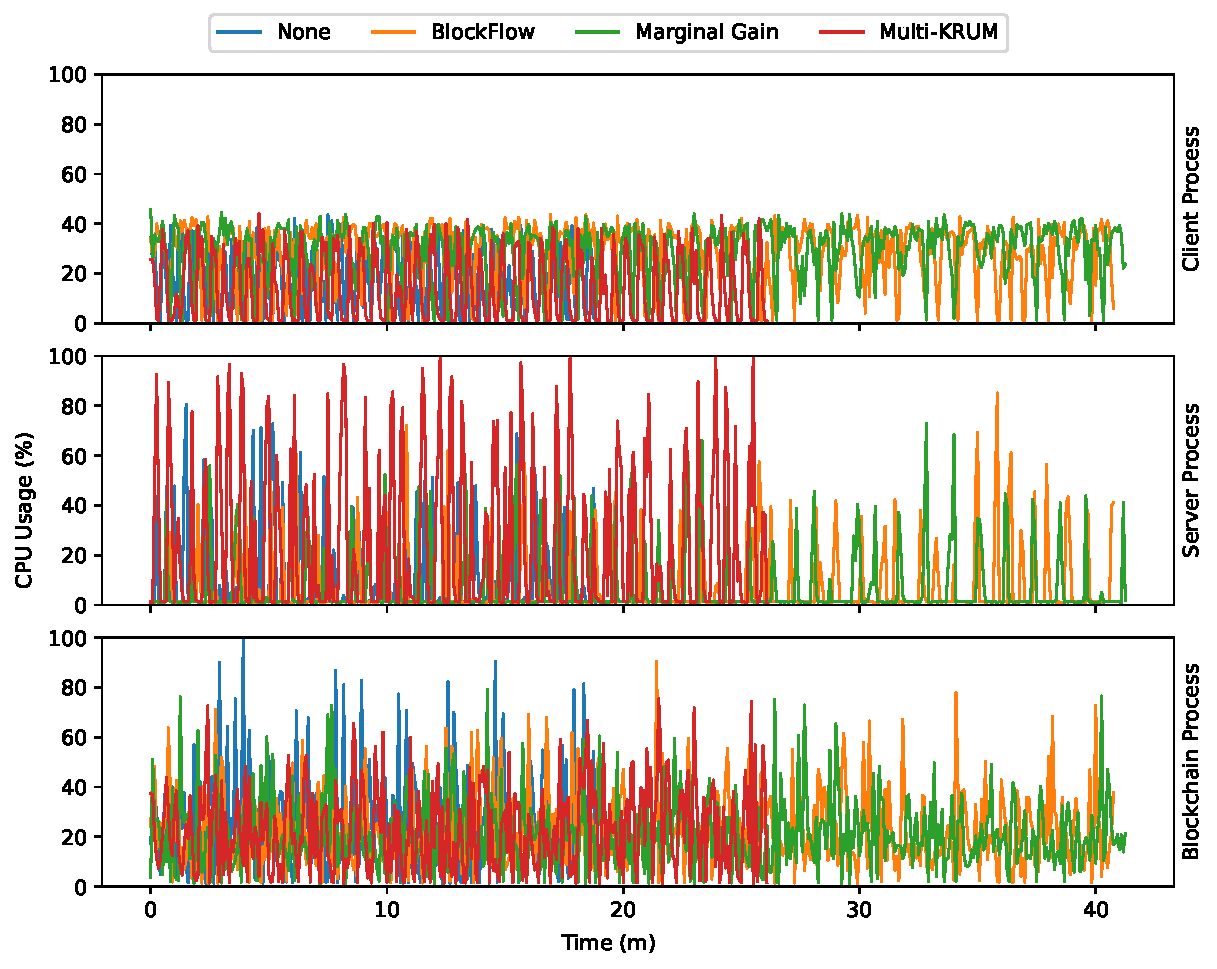
\includegraphics[width=0.8\textwidth]{graphics/scoring/cpu.pdf}
    \caption{CPU Usage Per Scoring Algorithm}
    \label{fig:cpu_scoring}
\end{figure}

\subsubsection{Conclusions and Improvements}

In conclusion, scoring algorithms that are executed on the clients, i.e.,the Marginal Gain and BlockFlow, have a higher impact on the overall system, leading to longer experiment execution times and higher resource usage for the clients. In contrary, algorithms that are executed on the servers, i.e., the Multi-KRUM, have a higher impact on the servers. Since there is usually a much higher number of clients than servers, the scoring algorithms executed by the servers have less impact on the overall system than the former. Additionally, the Marginal Gain was the most well performing algorithm in terms of model accuracy and convergence speed, followed by the Multi-KRUM and the BlockFlow.

If we had to choose an algorithm, the choices come down to the priorities of the system. If we are working with a system with resource-constrained devices, such as IoT systems, it is important that the impact on the clients is low. Therefore, scoring algorithms that run on the server, such as the Multi-KRUM, are more valuable. If the opposite is true, or if the resource consumption at the client is not relevant, the Marginal Gain could be chosen as it provides the best accuracy of the three.

It is also important to mention that algorithms that require more network traffic per round may be slower on clients with low bandwidth, which is the case of many IoT networks. With lower bandwidths, less traffic can go through at any point in time. Therefore, in case of high network traffic required during a round, devices with low bandwidth can make the process slower.

As a future improvement, servers can cache the client's update weights. Specifically, in case of the Multi-KRUM algorithm, the servers can download each of the client's submission twice: one time for scoring, one time for aggregating. However, the weights downloaded both times are the same as they are part of the same round. Therefore, caching can work well in favor of reducing the network traffic at the server for scoring algorithms that are executed by servers.

\subsection{Number of Clients}\label{horizontal:number_of_clients}

In this section, we analyze the impact of different numbers of clients on the scoring algorithms. For this comparison, all properties of the system are fixed, except for the amount of clients, which varies between 5, 10, 25 and 50, per each scoring algorithm.

\subsubsection{Execution Time, Transaction Cost, and Transaction Latency}

\autoref{fig:clients_metrics} illustrates the execution times, as well as the transaction latency and costs. The execution times of all scoring algorithms increase with the number of clients. However, they do not increase the same way. The Multi-KRUM algorithm, as well as not using any scoring algorithm, have a smaller execution time increase with the number of clients, when compared to BlockFlow and Marginal Gain. This can be explained by the fact that, in BlockFlow and Marginal Gain, the scorers are the clients. Since, as previously discussed, there are more clients than servers, the smart contract has to wait for more scorers to submit their scores, than it would have to wait when using Multi-KRUM. Consequently, the execution time increase with the number of devices is higher with scoring algorithms executed by the clients.

\begin{figure}[!ht]
    \centering
    \begin{subfigure}[b]{0.49\textwidth}
        \centering
        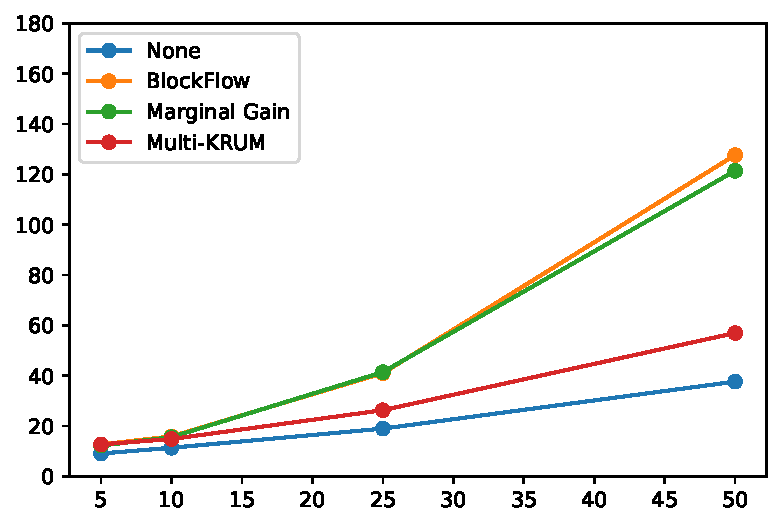
\includegraphics[width=\textwidth]{graphics/clients/e2e.pdf}
        \caption{E2E Time}
    \end{subfigure}
    \hfill
    \begin{subfigure}[b]{0.49\textwidth}
        \centering
        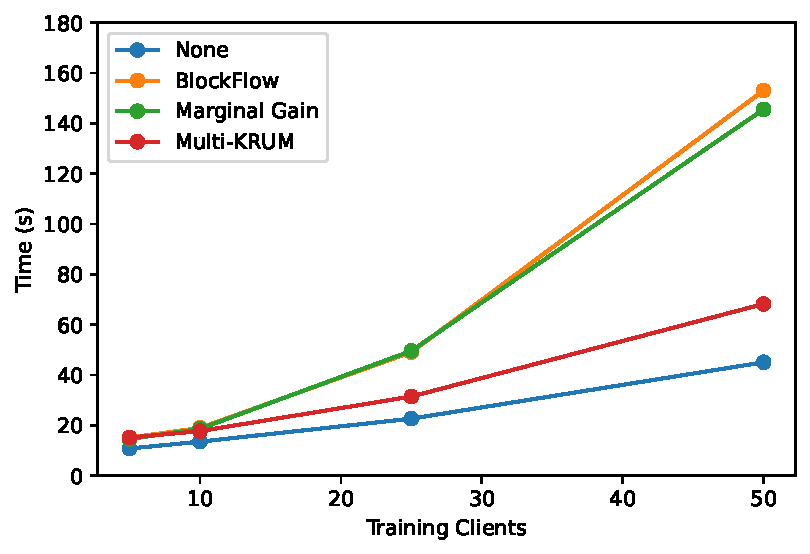
\includegraphics[width=\textwidth]{graphics/clients/round.pdf}
        \caption{Mean Round Time}
    \end{subfigure}
    \hfill
    \begin{subfigure}[b]{0.49\textwidth}
        \centering
        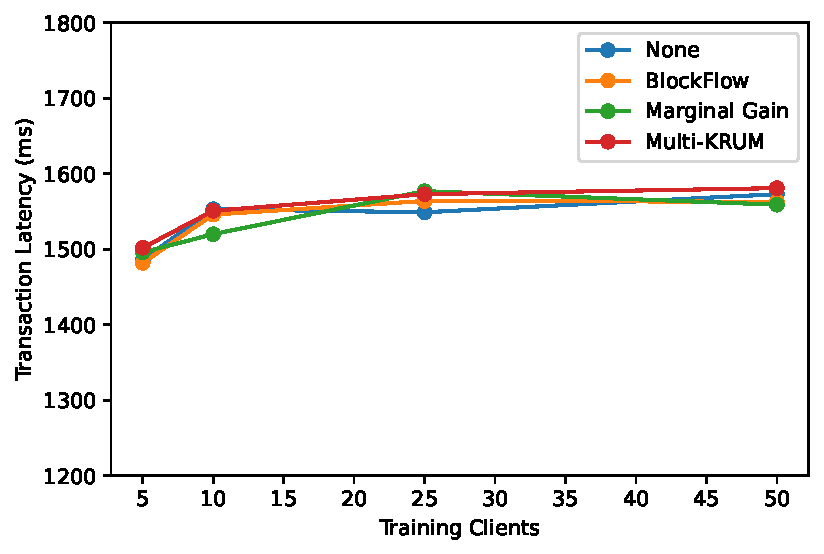
\includegraphics[width=\textwidth]{graphics/clients/tx_latency.pdf}
        \caption{Mean Transaction Latency}
    \end{subfigure}
    \hfill
    \begin{subfigure}[b]{0.49\textwidth}
        \centering
        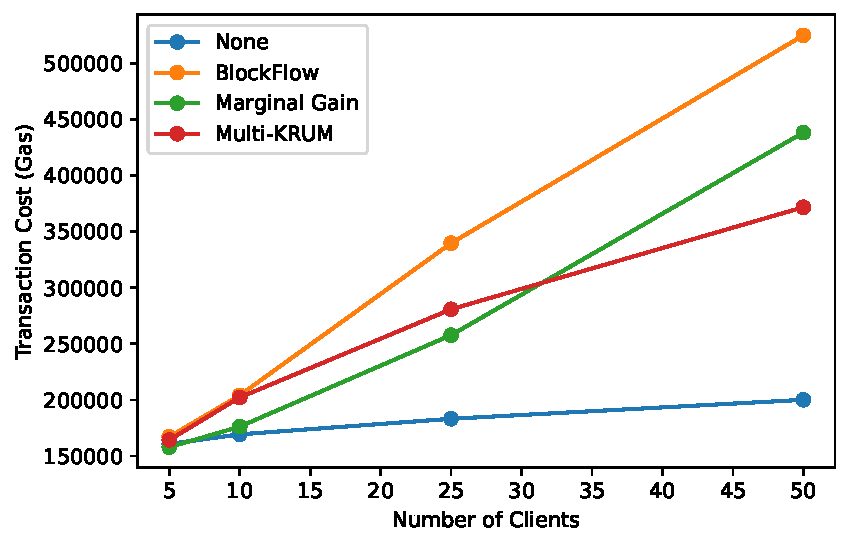
\includegraphics[width=\textwidth]{graphics/clients/tx_cost.pdf}
        \caption{Mean Transaction Cost}
    \end{subfigure}
    \caption{Execution Time, Transaction Cost, and Transaction Latency Per Number of Clients}
    \label{fig:clients_metrics}
\end{figure}

Regarding the transaction latency, there is no significant change with the variation of number of clients. As discussed before, transaction latency is mostly determined by the capacity of the network to handle the transactions. The Ethereum has a relatively fixed capacity of transactions per second of around 15 transactions per second. Our system alone does not reach that rate of transactions, not influencing the transaction latency. It is worth pointing out that, if the number of clients was in the order of hundreds, leading to elevated number of transactions, the latency would likely increase.

Regarding the transaction costs, we observe that they increase with the increased number of clients. In addition, the transaction costs growth is similar per algorithm. Firstly, we can calculate how many transactions we incur per algorithm per round by $T+A+S$, where $T$ is the number of trainers, usually clients, $A$ is the number of aggregators, usually servers, and $S$ the number of scorers, which can be either the clients or servers. When no scoring algorithm is used, the system only requires $T+A$ transactions, where $T$ is the number of clients and the only growing variable. With the Multi-KRUM, the system requires $T+2A$ transactions, since $S=A$, leading to a faster growth than when no scoring algorithm is used. Finally, both BlockFlow and Marginal Gain algorithms require $2T+A$ transactions and since $T > A$ and $T$ is the number of growing clients, it is also expected that the transaction cost would increase more than for the Multi-KRUM.

\subsubsection{Model Accuracy and Convergence}

As it can be seen from \autoref{fig:accuracy_clients}, the model accuracy and how it converges varies differently with different scoring algorithms. Overall, we observe that lower number of clients leads to a less stable convergence, represented by the spiking in the model accuracy plots. With a low number of clients, such as 5, the selected number of clients per round is also low due to the random way the participant selection algorithms chooses how many clients participate per round. Therefore, the model is trained with less diverse data per round. Consequently, the model can skew at some points during training, leading to a less stable convergence. In contrary, using more clients, namely 25 and 50, has an overall positive effect on both convergence stability and convergence speed. This is also likely related to the fact that the model is trained with more diverse samples from more clients in each round, leading to a better results.

\begin{figure}[!ht]
    \centering
    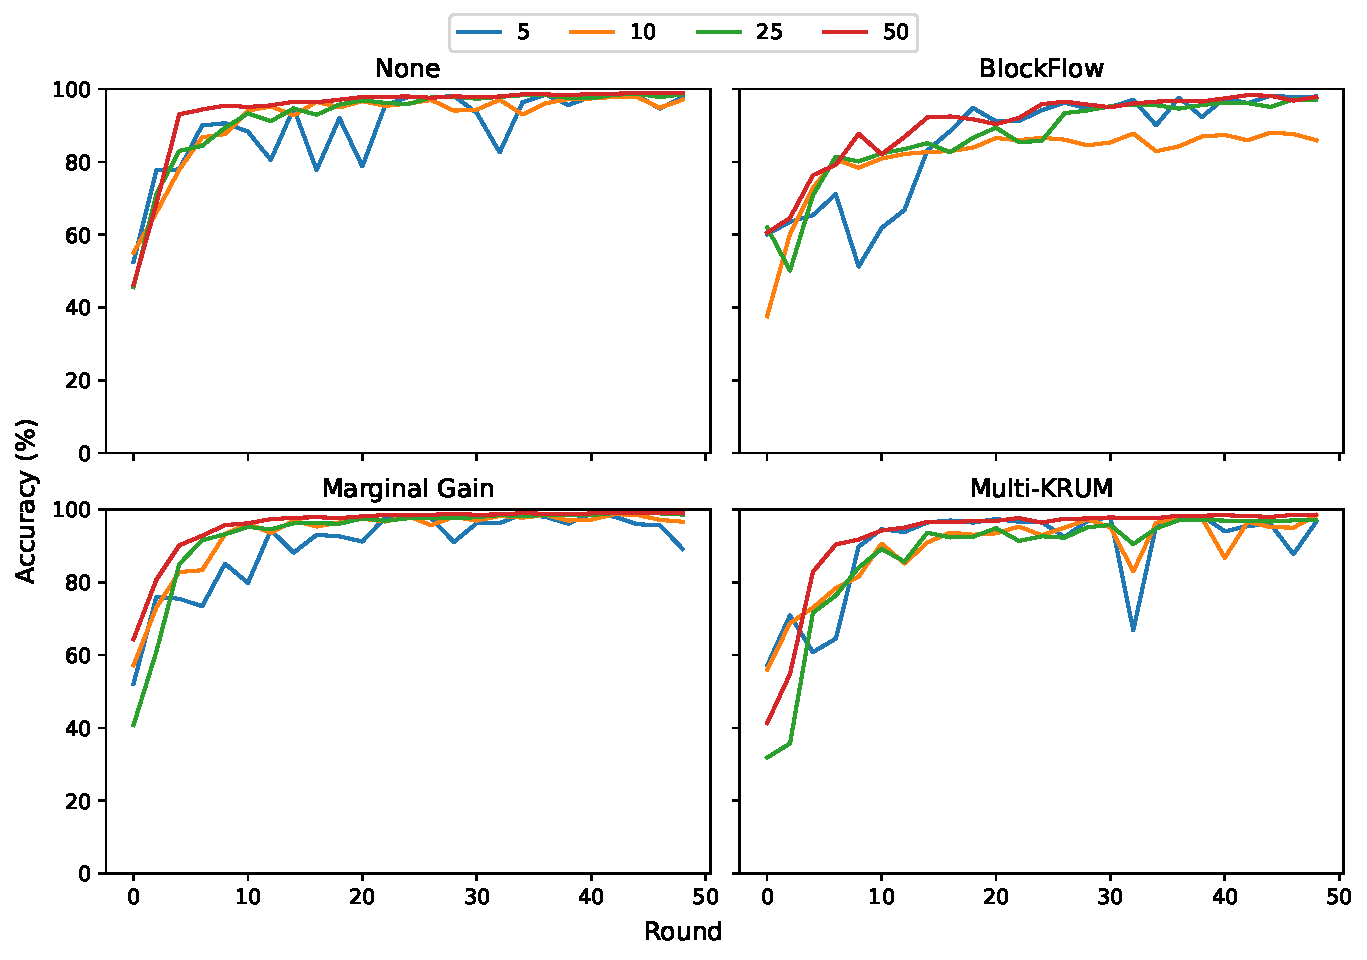
\includegraphics[width=\textwidth]{graphics/clients/accuracy.pdf}
    \caption{Model Accuracy Per Number of Clients}
    \label{fig:accuracy_clients}
\end{figure}

When it comes to the algorithm that performs best, the conclusions drawn from \Cref{horizontal:scoring_overall} remain true: the Marginal Gain performs the best, followed by the Multi-KRUM and finally by the BlockFlow.

\subsubsection{Communication Costs}

As it can be seen from \autoref{fig:net_clients}, the communication costs vary with the number of clients. Firstly, we observe that in terms of incoming traffic at the client process, there are significant differences depending on the scoring algorithm used.

\begin{figure}[!ht]
    \centering
    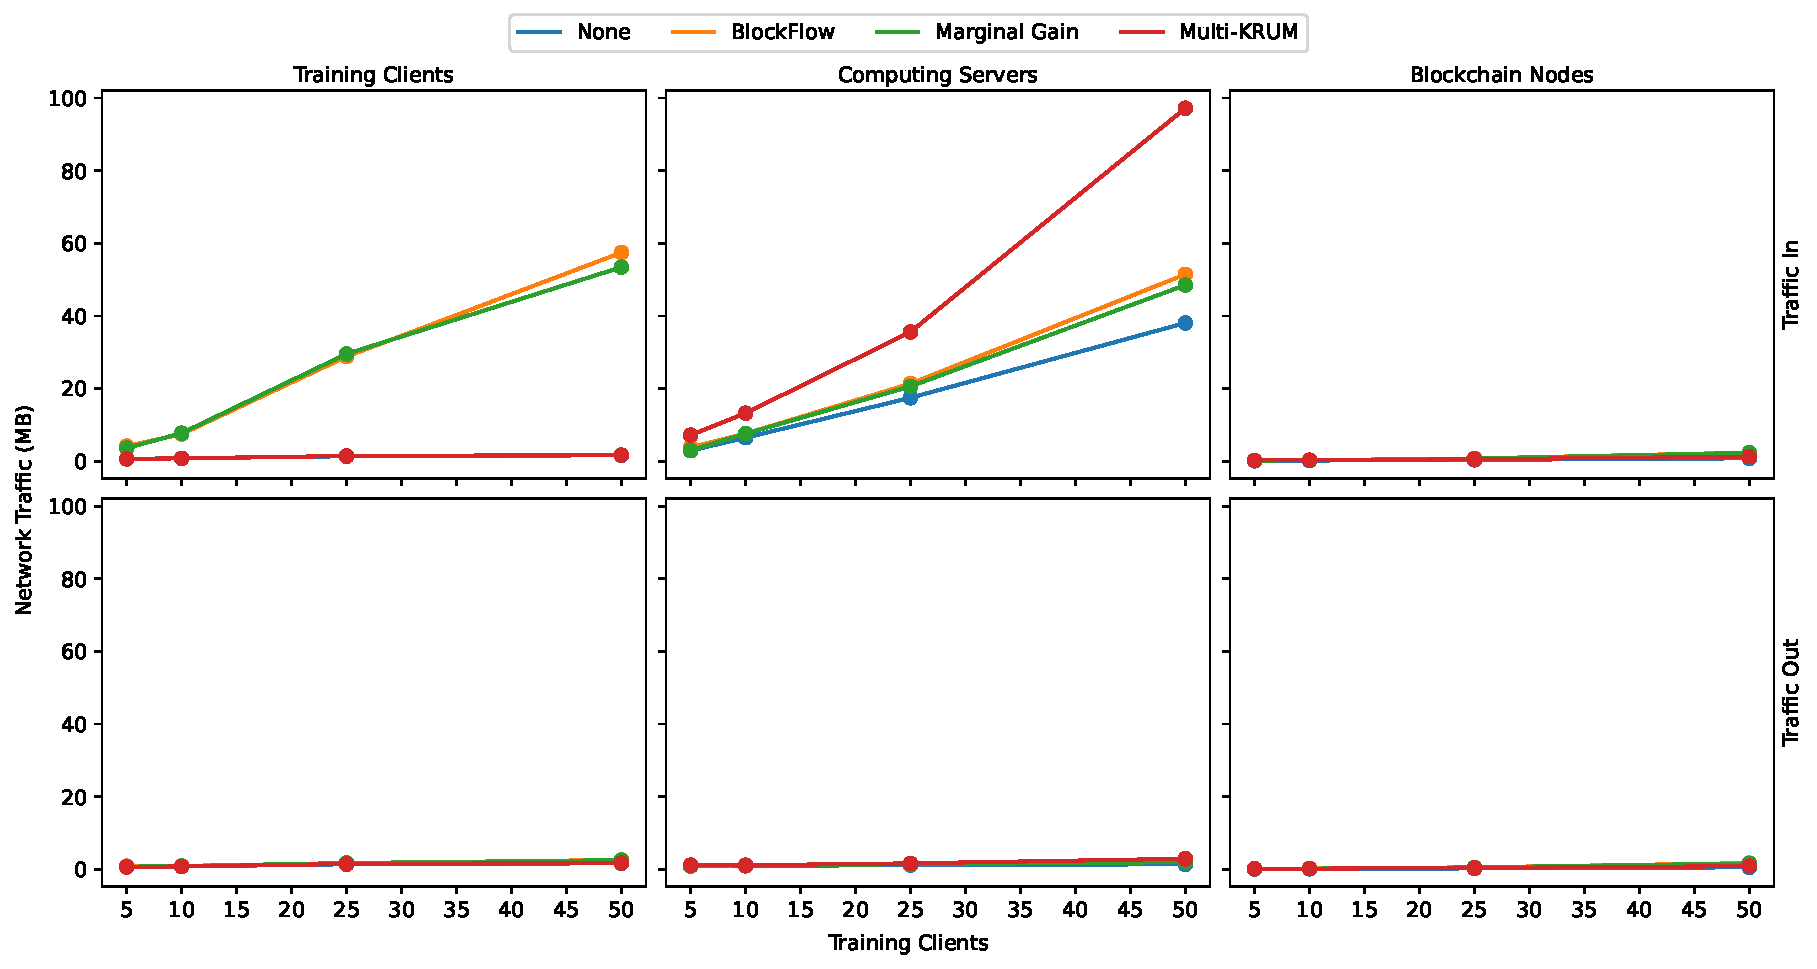
\includegraphics[width=\textwidth]{graphics/clients/traffic.pdf}
    \caption{Network Traffic Per Number of Clients}
    \label{fig:net_clients}
\end{figure}

One may notice that incoming traffic at the clients only increases when using scoring algorithms that are executed by the clients, such as the BlockFlow and the Marginal Gain. This can be explained by the fact that the more clients means the more weights from these clients need to be downloaded and scored. In contrary, when the scoring algorithm is executed by the server, there are virtually no changes in the incoming traffic when number of clients is increased. This is because the client only has to download the global weights after each round, which is not influenced by the number of clients.

Secondly, we observe that the incoming traffic always grows linearly at the servers when using a scoring algorithm that runs at the clients. However, when using a algorithm that runs on the server, such as the Multi-KRUM, the growth is higher than for the remaining algorithms. In all cases, the servers always have to download the weights for aggregation. However, if the scoring is executed at the servers, they will download the weights twice as explained in \Cref{horizontal:scoring_overall}, leading to a super-linear traffic growth. As previously suggested, this can be improved by caching the weights between these two phases.

Thirdly, we observe that the outgoing traffic differences are not significant for any of the processes. Regarding the clients and servers, we observe a very small increase on the client or server processes, if the scoring algorithm is executed by the clients or servers, respectively. However, the differences of outgoing traffic per number of clients for each scoring algorithm are negligible.

Finally, the differences observed in the blockchain process, both for incoming and outgoing traffic are negligible. With the increase of the number of clients, there are more transactions going through the blockchain. However, the transactions on the blockchain are very small when compared to the size of weights that need to be uploaded and downloaded by the clients and servers, respectively.

\subsubsection{Computation Costs}

\autoref{fig:ram_clients_clients}, \autoref{fig:ram_clients_servers}, \autoref{fig:ram_clients_miners} show the RAM usage at the clients, servers, and blockchain processes, while  \autoref{fig:cpu_clients_clients}, \autoref{fig:cpu_clients_servers}, \autoref{fig:cpu_clients_miners} show the CPU usage at the clients, servers, and blockchain processes, respectively. Overall, it can be seen that the number of clients has no major impact on RAM and CPU usage of either clients or servers.

Even though the usage of RAM and CPU at a certain points in time does not vary significantly, some scoring algorithms have more impact on the clients, or on the servers, as discussed in \Cref{horizontal:scoring_overall}. In addition, we observe that the increase of resource usage is proportional to the number of clients, depending on whether the the scoring algorithm is executed by the clients or the servers.

The only major change is observed in the RAM and CPU usage of the blockchain process. The higher the number of clients, the higher the RAM and CPU usage. This is expected as more clients are connected to the blockchain, meaning that more devices continuously interact and send transactions to the blockchain.

\subsubsection{Conclusions and Improvements}

In conclusion, scoring algorithms executed by the clients, i.e., the BlockFlow and Marginal Gain, show higher execution time increases with respect to the number of clients. In addition, the resource usage at the clients increases linearly with the number of devices. In contrary, algorithms executed by the servers, i.e., the Multi-KRUM, do not have significant effects on the clients' resources usage. Therefore, in systems with resource-constrained clients, algorithms executed by the server may be the ideal solution.

Finally, the resource usage of the blockchain process, mainly in terms of RAM, increases with the number of clients. The blockchain resource usage is an important aspect to consider in BFS systems. There is a clear trade-off between the number of clients with the blockchain resource usage.

\subsection{Privacy Degrees}

In this section, we analyze the impact of different privacy degrees on each scoring algorithm. In this set of experiments, all properties of the system are fixed, except for the degree of privacy, which varies between 0, 1 and 5, per each scoring algorithm.

\subsubsection{Execution Time, Transaction Cost, and Transaction Latency}

As it can be seen from \autoref{fig:priv_metrics}, having a privacy mechanism increases the execution time of each round by approximately $16.6$ seconds. In addition, the privacy degree itself does not seem to influence the execution time significantly.

Regarding the transaction latency and costs, there are no significant differences. The privacy mechanism is executed by the clients before they submit their model update, and does not change the number of transactions. Consequently, it has no impact on the blockchain process itself.

\begin{figure}[!hpt]
    \centering
    \begin{subfigure}[b]{0.47\textwidth}
        \centering
        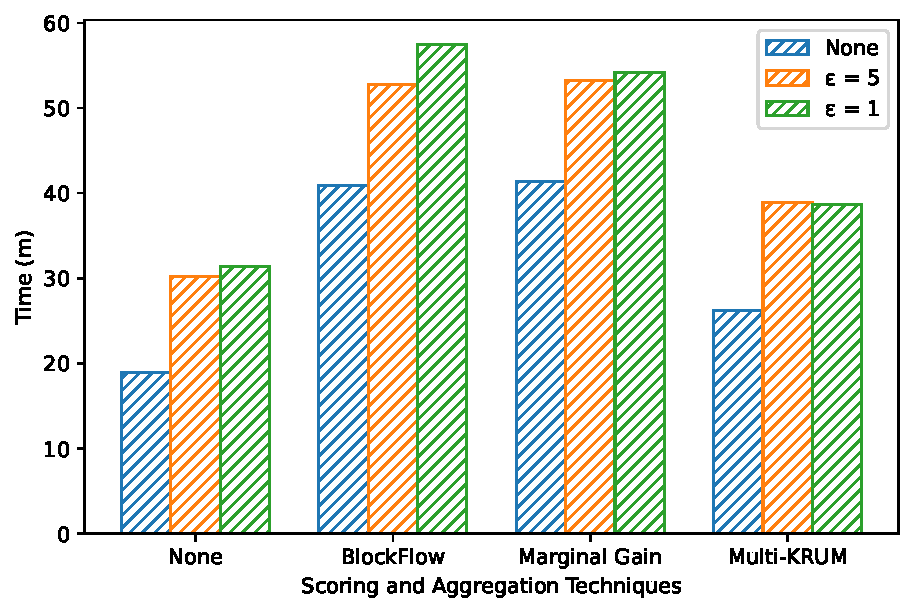
\includegraphics[width=\textwidth]{graphics/privacy/e2e.pdf}
        \caption{E2E Time}
    \end{subfigure}
    \hfill
    \begin{subfigure}[b]{0.47\textwidth}
        \centering
        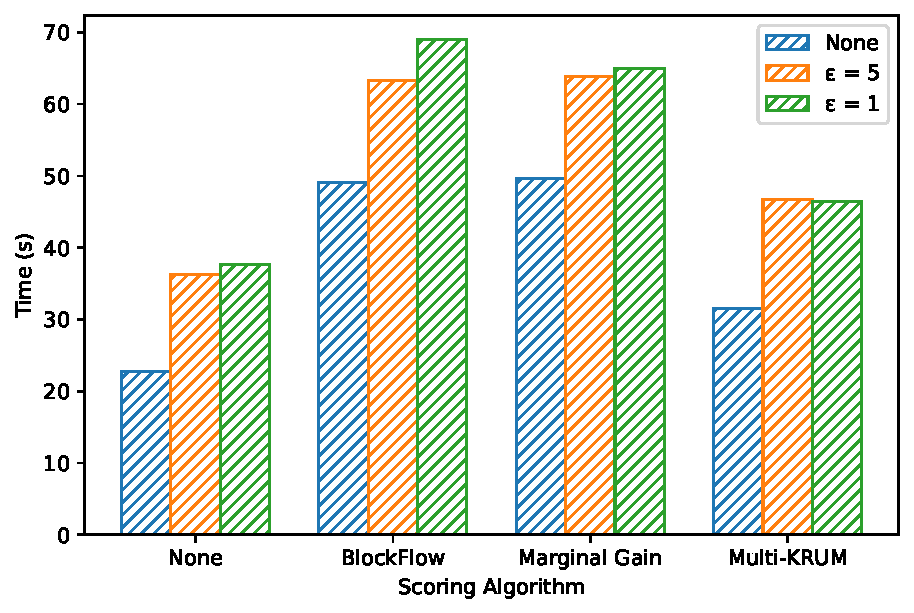
\includegraphics[width=\textwidth]{graphics/privacy/round.pdf}
        \caption{Mean Round Time}
    \end{subfigure}
    \hfill
    \begin{subfigure}[b]{0.47\textwidth}
        \centering
        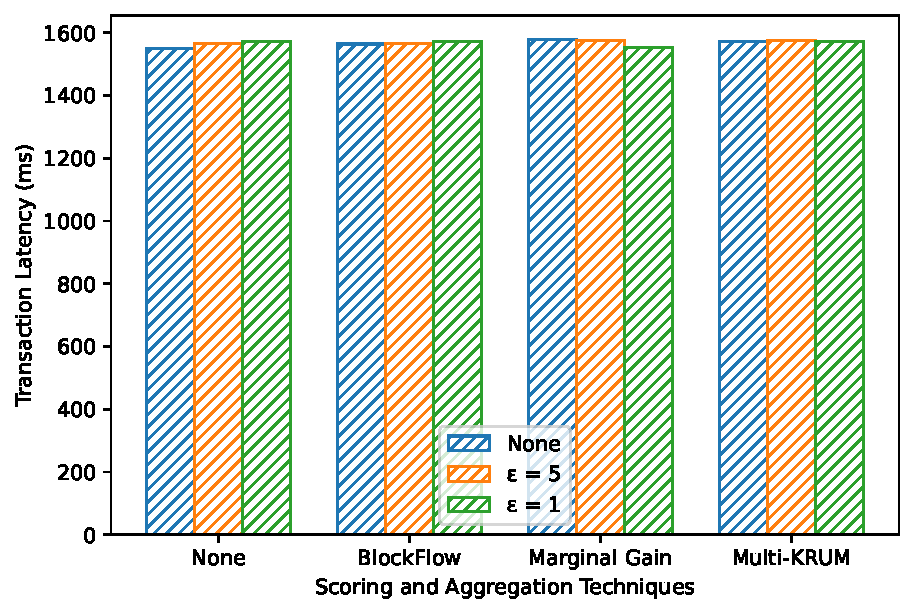
\includegraphics[width=\textwidth]{graphics/privacy/tx_latency.pdf}
        \caption{Transaction Latency}
    \end{subfigure}
    \hfill
    \begin{subfigure}[b]{0.47\textwidth}
        \centering
        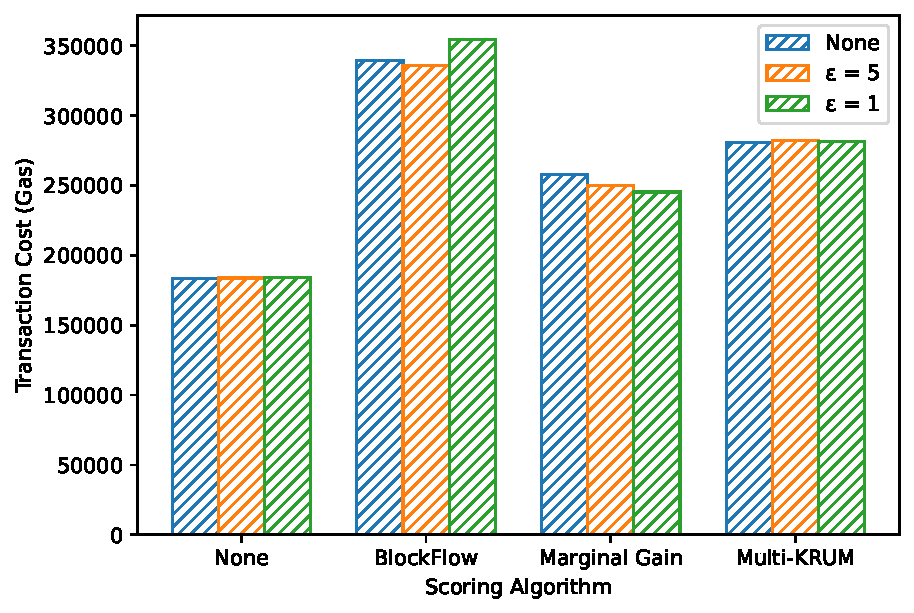
\includegraphics[width=\textwidth]{graphics/privacy/tx_cost.pdf}
        \caption{Transaction Cost}
    \end{subfigure}
    \caption{Execution Time, Transaction Cost, and Transaction Latency Per Privacy Degree}
    \label{fig:priv_metrics}
\end{figure}

\begin{figure}[!hpb]
    \centering
    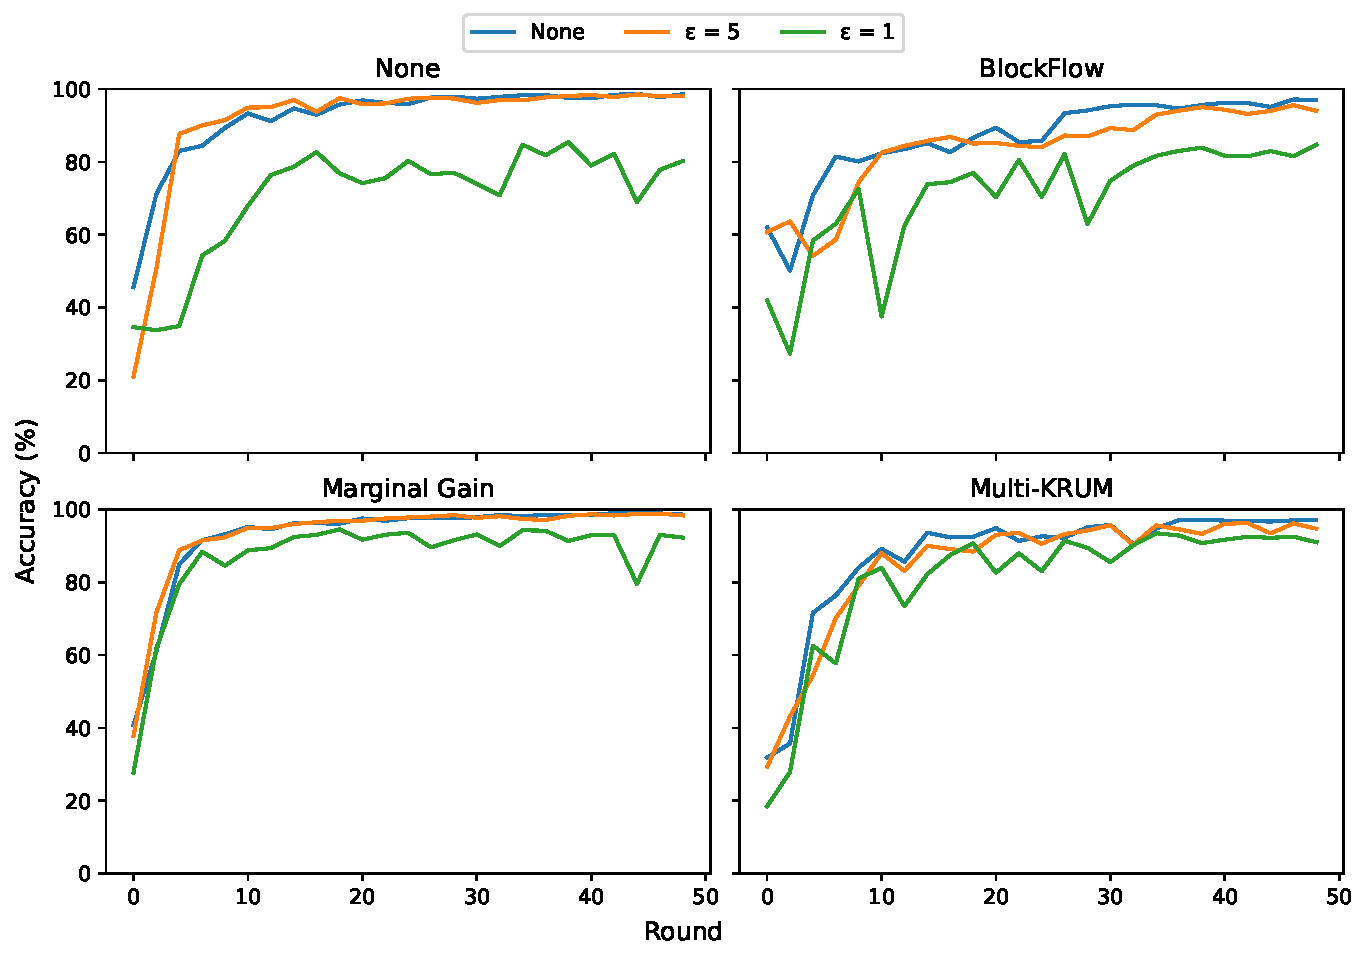
\includegraphics[width=\textwidth]{graphics/privacy/accuracy.pdf}
    \caption{Model Accuracy Per Privacy Degree}
    \label{fig:accuracy_privacy}
\end{figure}

\subsubsection{Model Accuracy and Convergence}

As it can be seen from \autoref{fig:accuracy_privacy}, different scoring algorithms have different accuracy drops using different privacy degrees. Overall, we observe that not using a scoring algorithm performs the worse with the highest degree of privacy, i.e., $\epsilon = 1$. In addition, a lower degree of privacy, i.e., $\epsilon = 5$, yields similar, yet lower, model accuracy than not using privacy degree. The higher the degree of privacy, the higher the noise values that are added to the original weights. Since the weights include added noise, it is expected that the accuracy will be lower with the higher degrees of privacy.

Out of the three scoring algorithms, the Marginal Gain and Multi-KRUM perform the best in presence of the higher degrees of privacy. As explained in \Cref{background:scoring}, both of these algorithms reject the worst updates, while BlockFlow does not. By rejecting the worst update, these algorithms always keep the best updates that provide the higher accuracy, even after noise is being added to the weights. Therefore, the Multi-KRUM and Marginal Gain have a lower accuracy drop with the higher privacy degrees, allowing them to maintain high model accuracy while preserving privacy.

\subsubsection{Communication Costs}

In terms of communication costs, as illustrated in \autoref{fig:net_privacy}, there are no significant differences depending on the privacy degree used. Adding noise to the weights does not necessarily increase their sizes and, for that reason, the network traffic costs are not expected to change significantly.

\begin{figure}[!h]
    \centering
    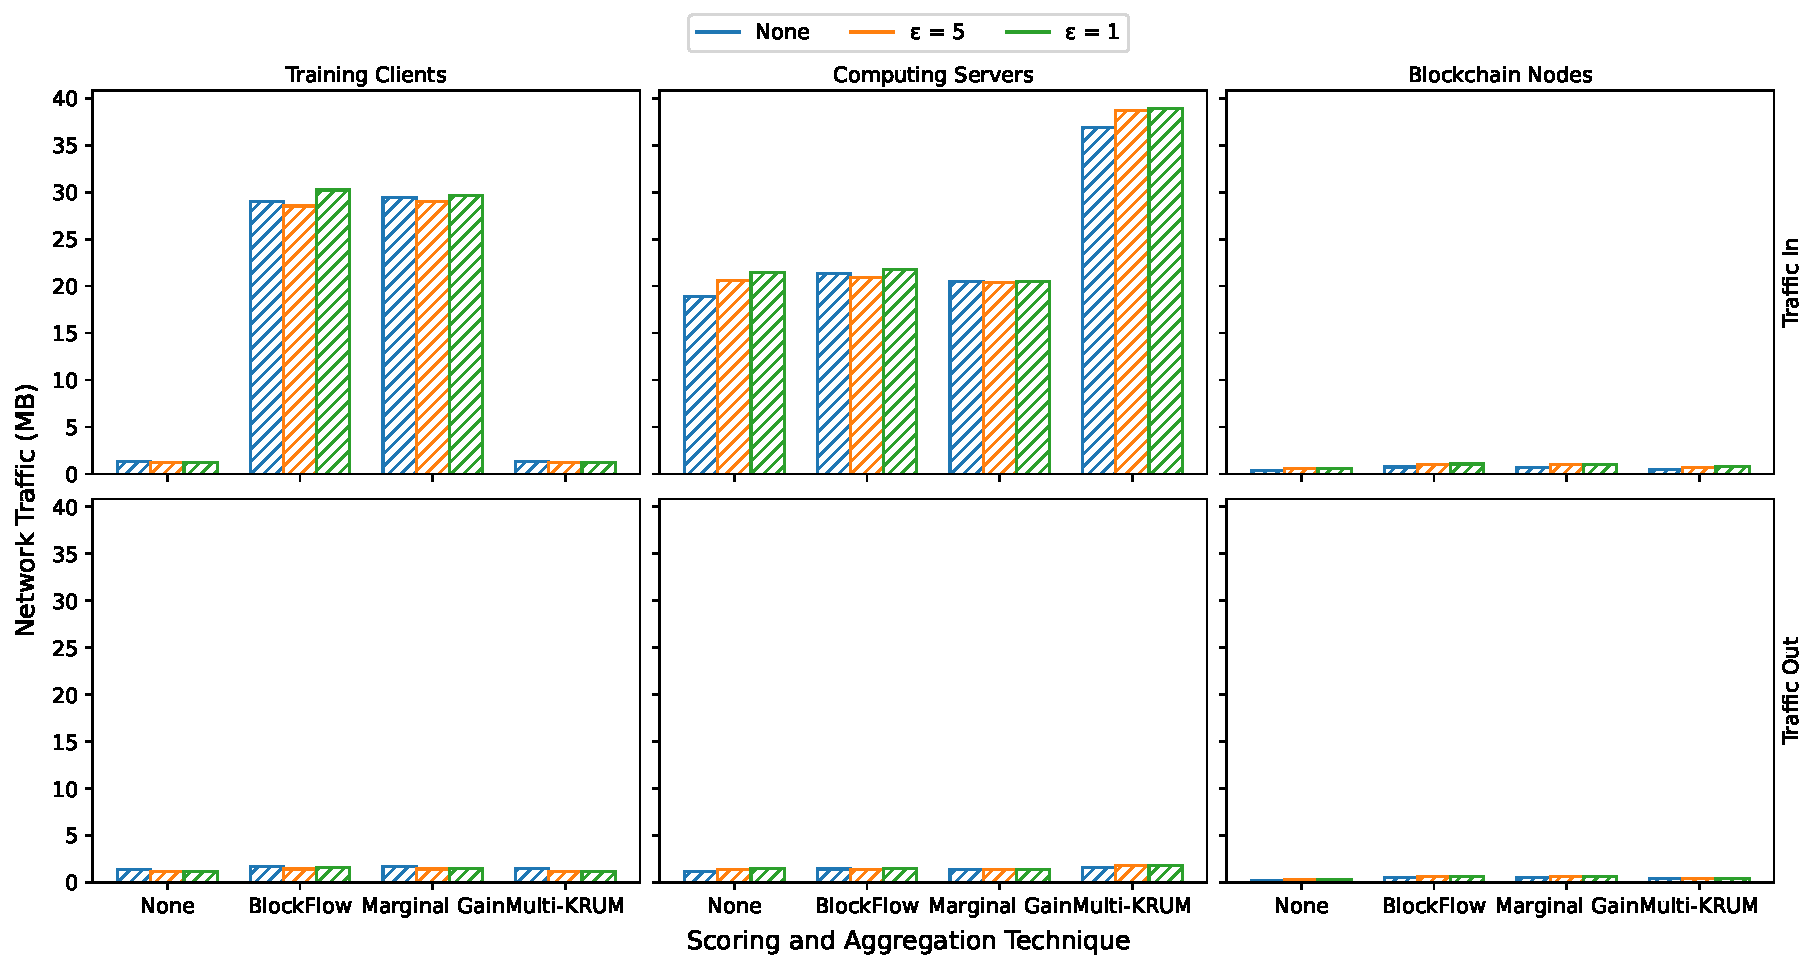
\includegraphics[width=\textwidth]{graphics/privacy/traffic.pdf}
    \caption{Network Traffic Per Privacy Degree}
    \label{fig:net_privacy}
\end{figure}

\subsubsection{Computation Costs}

\autoref{fig:ram_privacy_clients}, \autoref{fig:ram_privacy_servers}, \autoref{fig:ram_privacy_miners} show the RAM usage at the clients, servers, and blockchain processes, while \autoref{fig:cpu_privacy_clients}, \autoref{fig:cpu_privacy_servers}, \autoref{fig:cpu_privacy_miners} show the CPU usage at the clients, servers, and blockchain processes, respectively. Since the privacy algorithm is only executed by the client process, we only expect the computation costs, namely the CPU usage, to increase at the client process. Overall, we can observe that this is true as there are no significant changes in the RAM or CPU usage for the servers and blockchain processes.

As it can be seen from \autoref{fig:ram_privacy_clients}, the privacy mechanisms have no significant impact on RAM usage. The privacy algorithm has little RAM usage when compared to the total required for model training. In contrary, the CPU usage is higher, not necessarily in terms of usage percentage, but in terms of longer usage times. This can be seen from \autoref{fig:cpu_privacy_clients} and is explained by the time required for the execution of the privacy algorithm at the clients.

\subsubsection{Conclusions}

In conclusion, we see that using a privacy algorithm increases the computation costs, and consequently, the resource usage, at the clients. This leads to longer execution times as clients that need to process their weights and add noise to them. Therefore, there is a clear trade-off between execution time and privacy. However, increasing the privacy degree does not increase the execution time.

In addition, one may notice that increasing the privacy degree leads to the lower model accuracy. This is expected since the privacy algorithm used introduce noise to the weights. However, some of the scoring algorithms are still able to achieve higher model accuracy values even with higher privacy degrees. This is the case for the Marginal Gain and Multi-KRUM, which are the most well-performing algorithms.

Finally, we can argue that adding a privacy preserving algorithm to a BFS system is crucial, specially if the model is trained with sensitive data. One of the main arguments to apply blockchain to a Federated Learning system is the traceability and auditability. To do so, the weights, or their representation in our case, are recorded in the blockchain, which means they are visible and retrievable by anyone in the network. This implies that there is a trade-off between traceability and auditability and the requirement for privacy mechanisms, which in turn leads to higher resource usage.

\clearpage

\begin{figure}[!h]
    \centering
    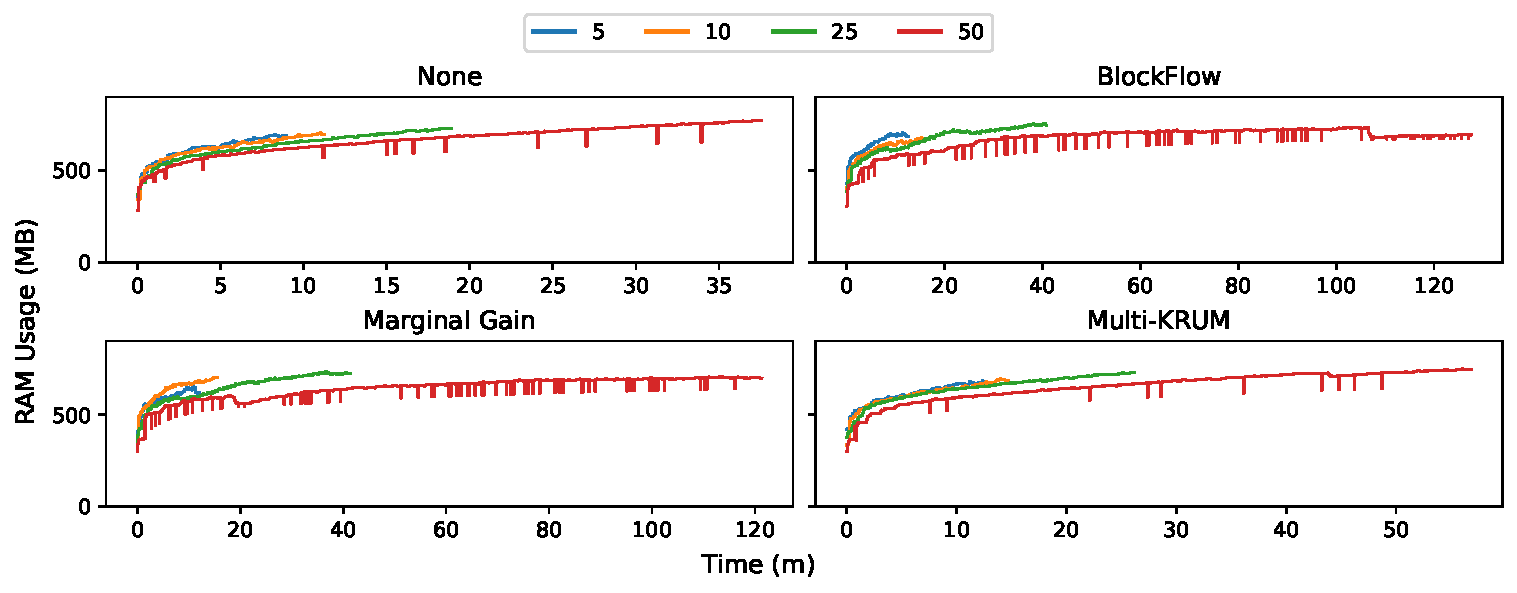
\includegraphics[width=\textwidth]{graphics/clients/ram_client.pdf}
    \caption{Client Process RAM Usage Per Number of Clients}
    \label{fig:ram_clients_clients}
\end{figure}

\vfill

\begin{figure}[!h]
    \centering
    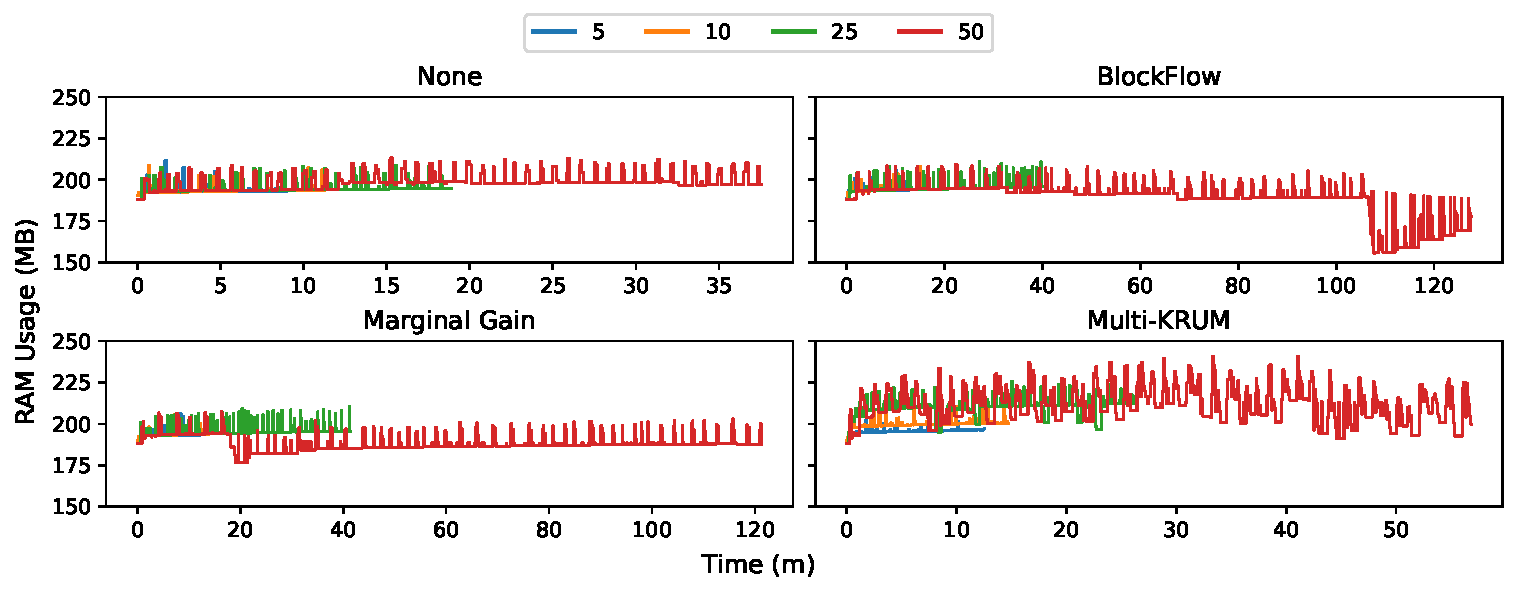
\includegraphics[width=\textwidth]{graphics/clients/ram_server.pdf}
    \caption{Server Process RAM Usage Per Number of Clients}
    \label{fig:ram_clients_servers}
\end{figure}

\vfill

\begin{figure}[!h]
    \centering
    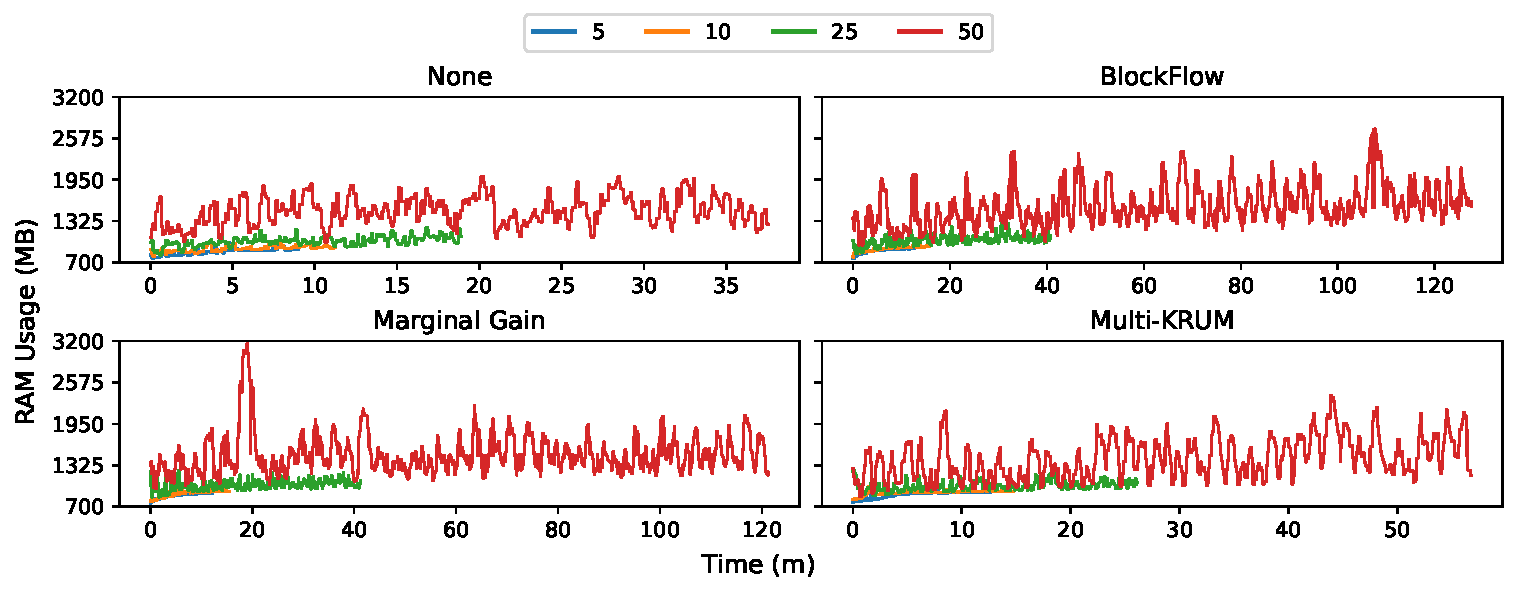
\includegraphics[width=\textwidth]{graphics/clients/ram_miner.pdf}
    \caption{Blockchain Process RAM Usage Per Number of Clients}
    \label{fig:ram_clients_miners}
\end{figure}

\clearpage

\begin{figure}[!h]
    \centering
    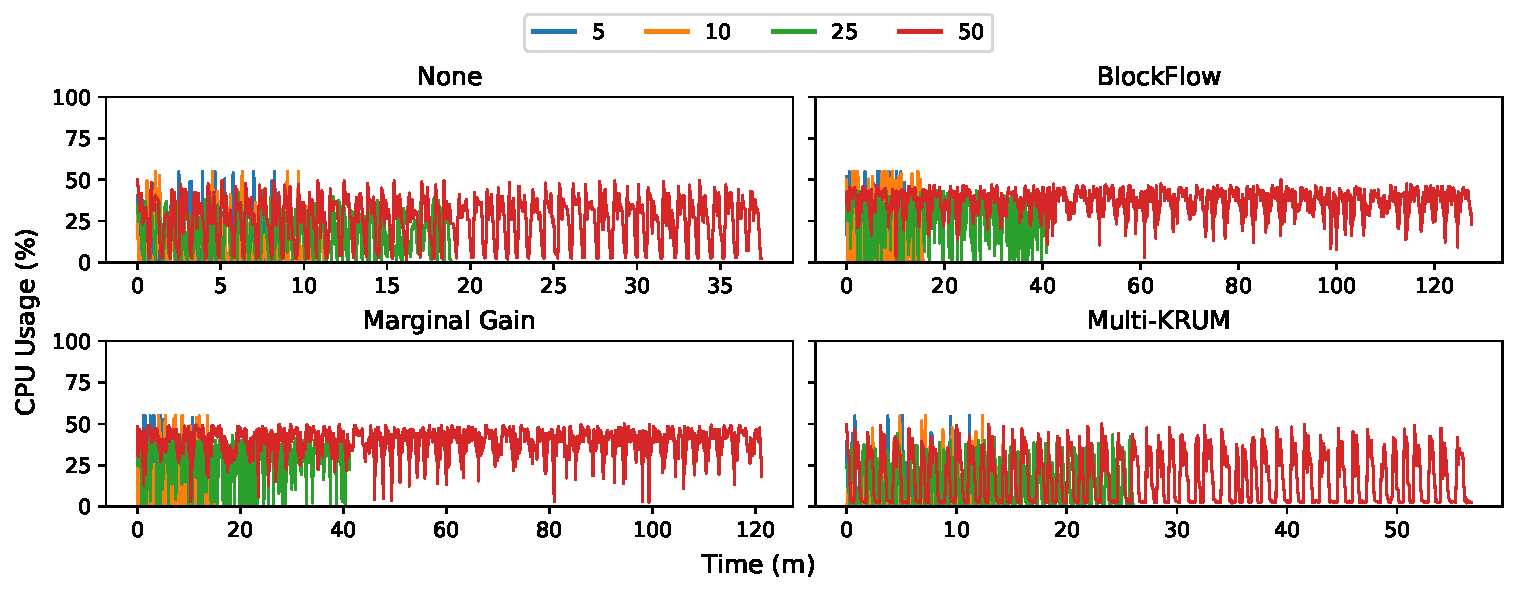
\includegraphics[width=\textwidth]{graphics/clients/cpu_client.pdf}
    \caption{Client Process CPU Usage Per Number of Clients}
    \label{fig:cpu_clients_clients}
\end{figure}

\vfill

\begin{figure}[!h]
    \centering
    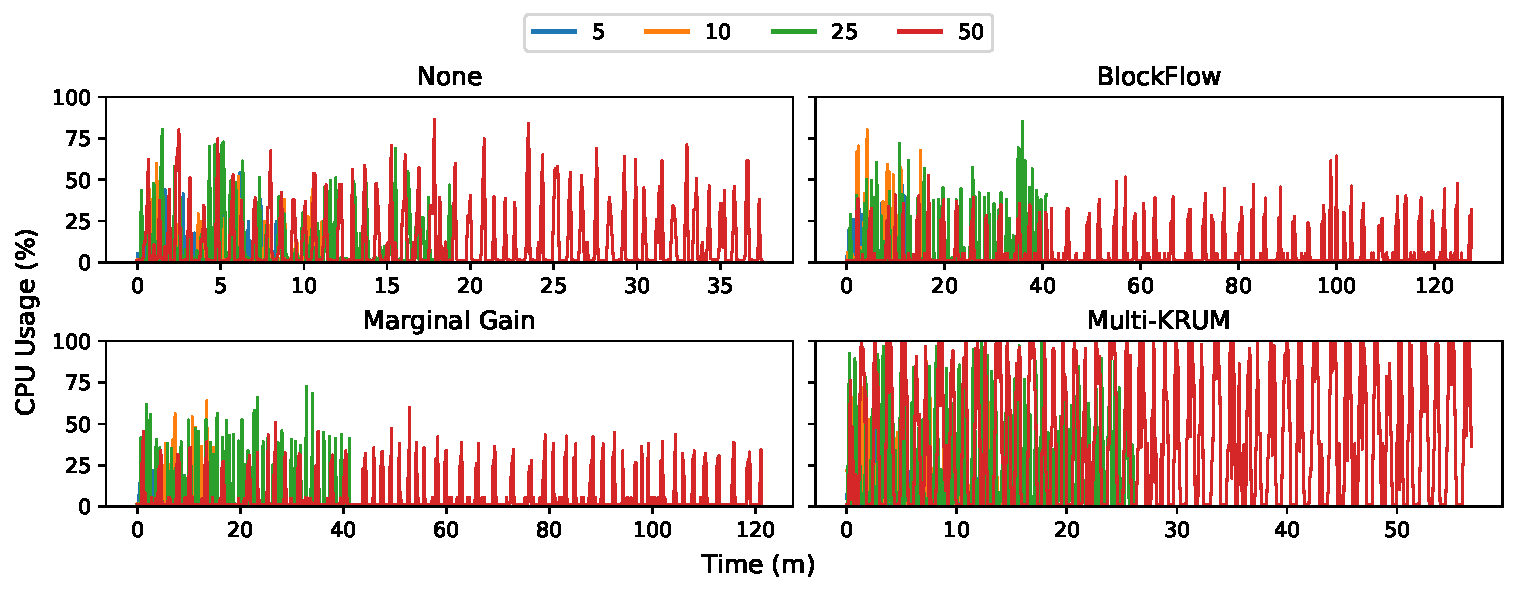
\includegraphics[width=\textwidth]{graphics/clients/cpu_server.pdf}
    \caption{Server Process CPU Usage Per Number of Clients}
    \label{fig:cpu_clients_servers}
\end{figure}

\vfill

\begin{figure}[!h]
    \centering
    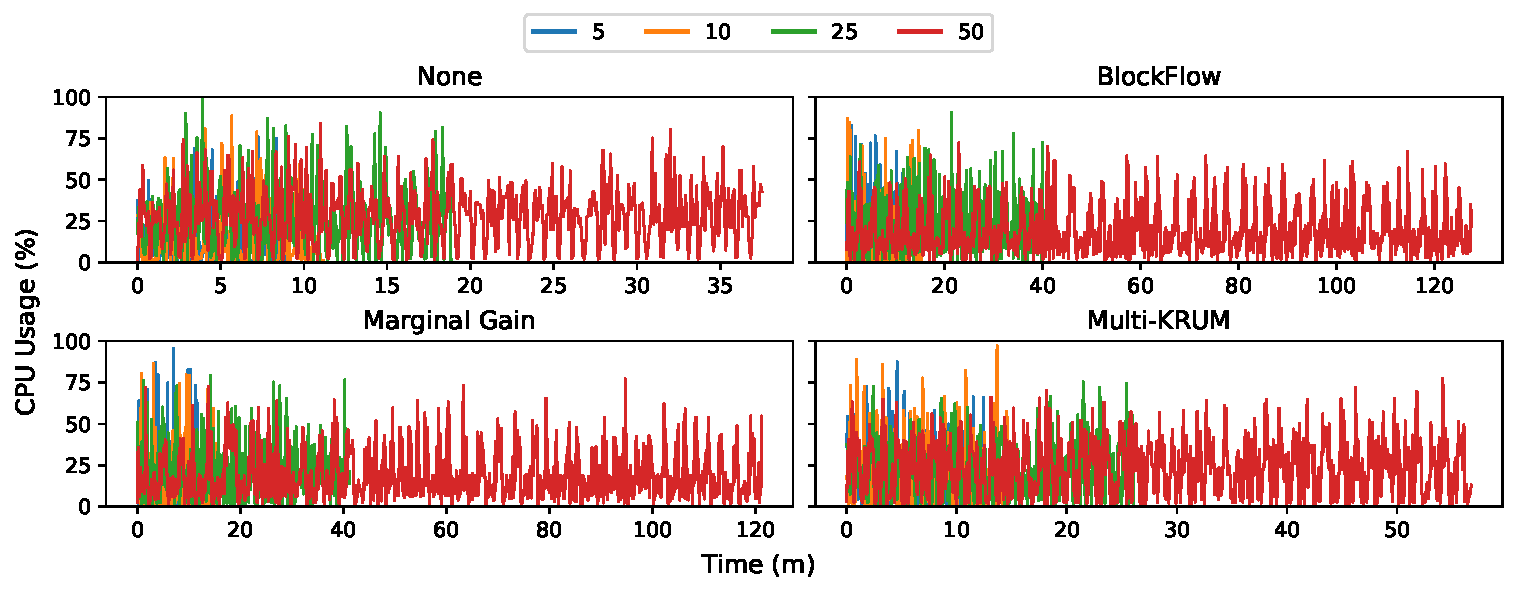
\includegraphics[width=\textwidth]{graphics/clients/cpu_miner.pdf}
    \caption{Blockchain Process CPU Usage Per Number of Clients}
    \label{fig:cpu_clients_miners}
\end{figure}

\clearpage

\begin{figure}[!h]
    \centering
    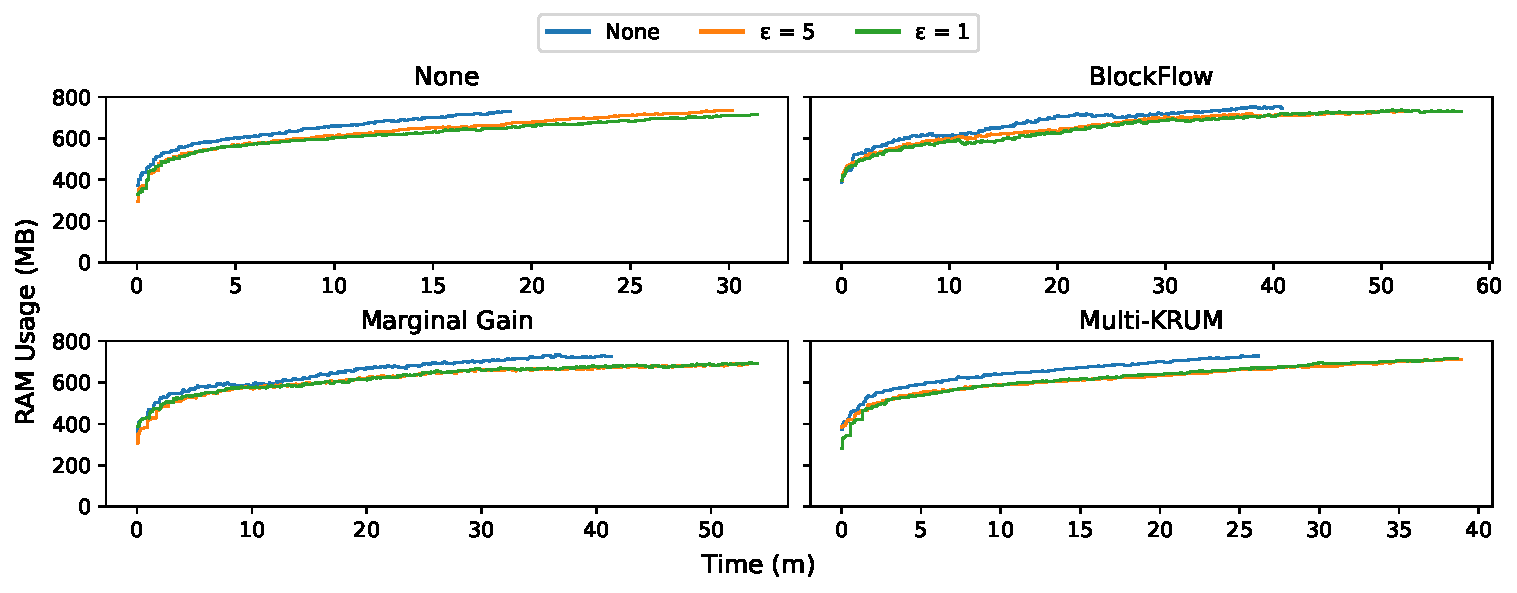
\includegraphics[width=\textwidth]{graphics/privacy/ram_client.pdf}
    \caption{Client Process RAM Usage Per Privacy Degree}
    \label{fig:ram_privacy_clients}
\end{figure}

\vfill

\begin{figure}[!h]
    \centering
    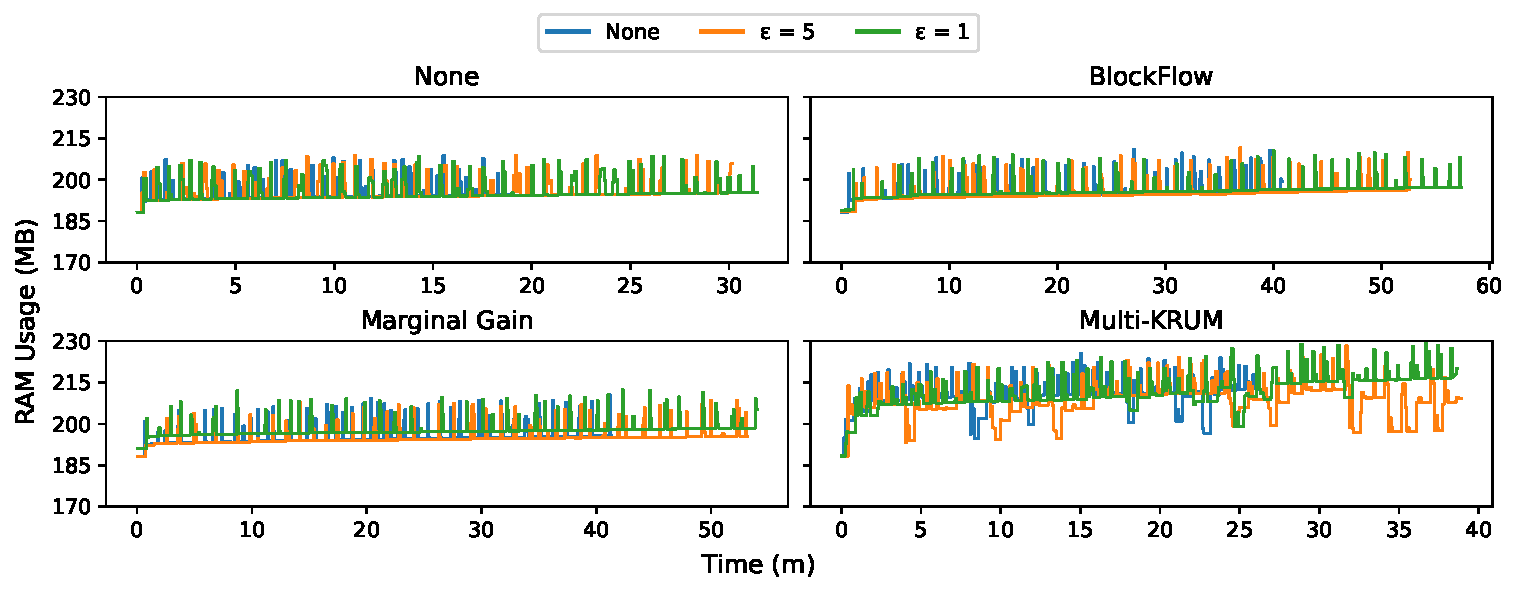
\includegraphics[width=\textwidth]{graphics/privacy/ram_server.pdf}
    \caption{Server Process RAM Usage Per Privacy Degree}
    \label{fig:ram_privacy_servers}
\end{figure}

\vfill

\begin{figure}[!h]
    \centering
    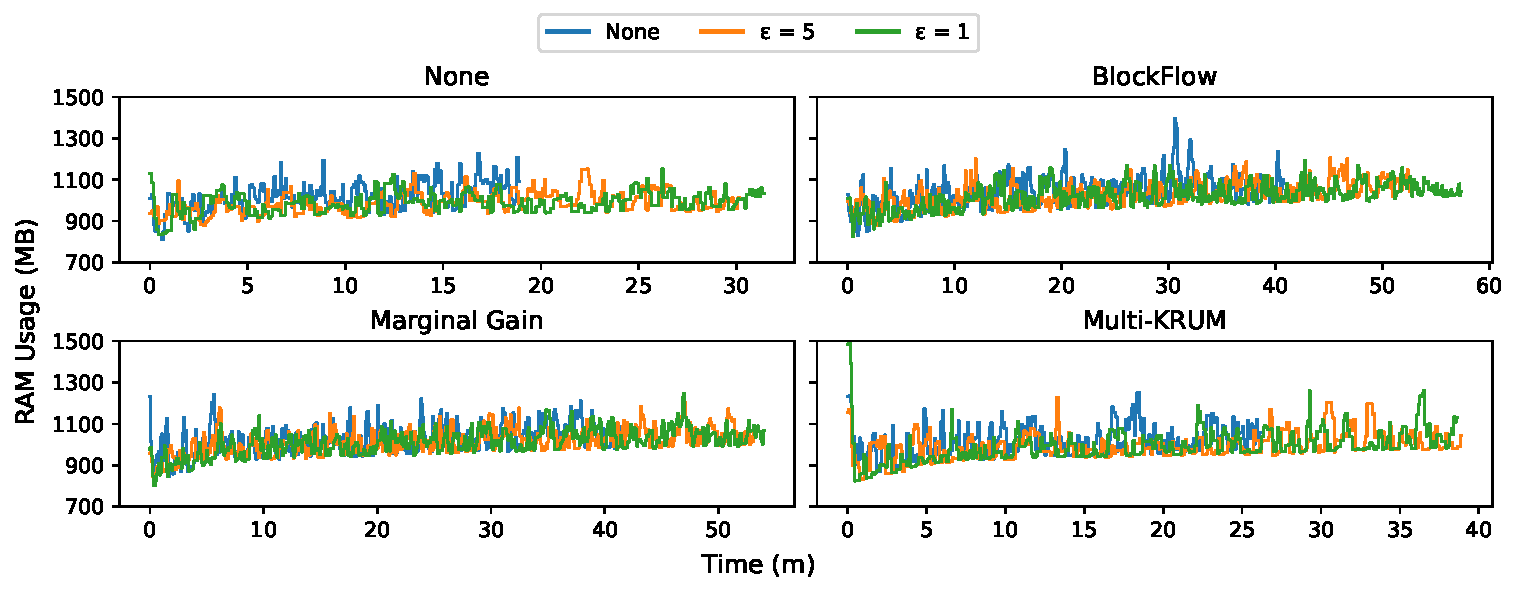
\includegraphics[width=\textwidth]{graphics/privacy/ram_miner.pdf}
    \caption{Blockchain Process RAM Usage Per Privacy Degree}
    \label{fig:ram_privacy_miners}
\end{figure}

\clearpage

\begin{figure}[!h]
    \centering
    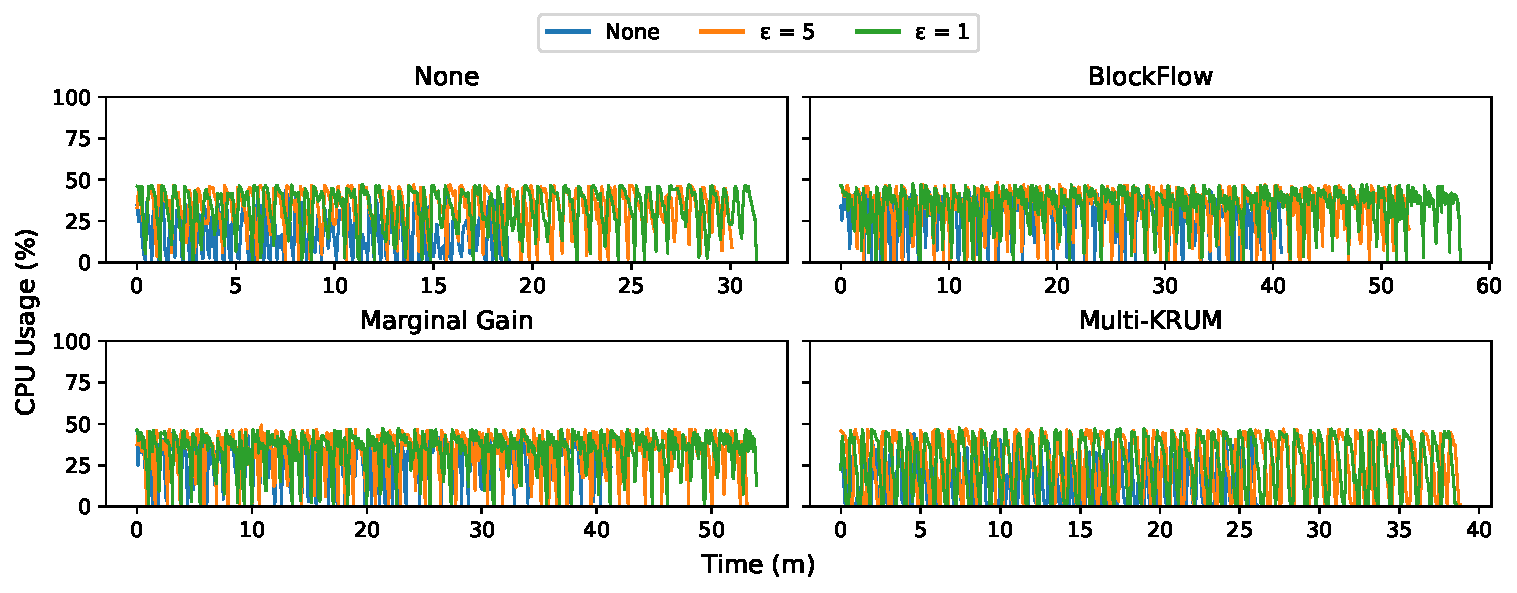
\includegraphics[width=\textwidth]{graphics/privacy/cpu_client.pdf}
    \caption{Client Process CPU Usage Per Privacy Degree}
    \label{fig:cpu_privacy_clients}
\end{figure}

\vfill

\begin{figure}[!h]
    \centering
    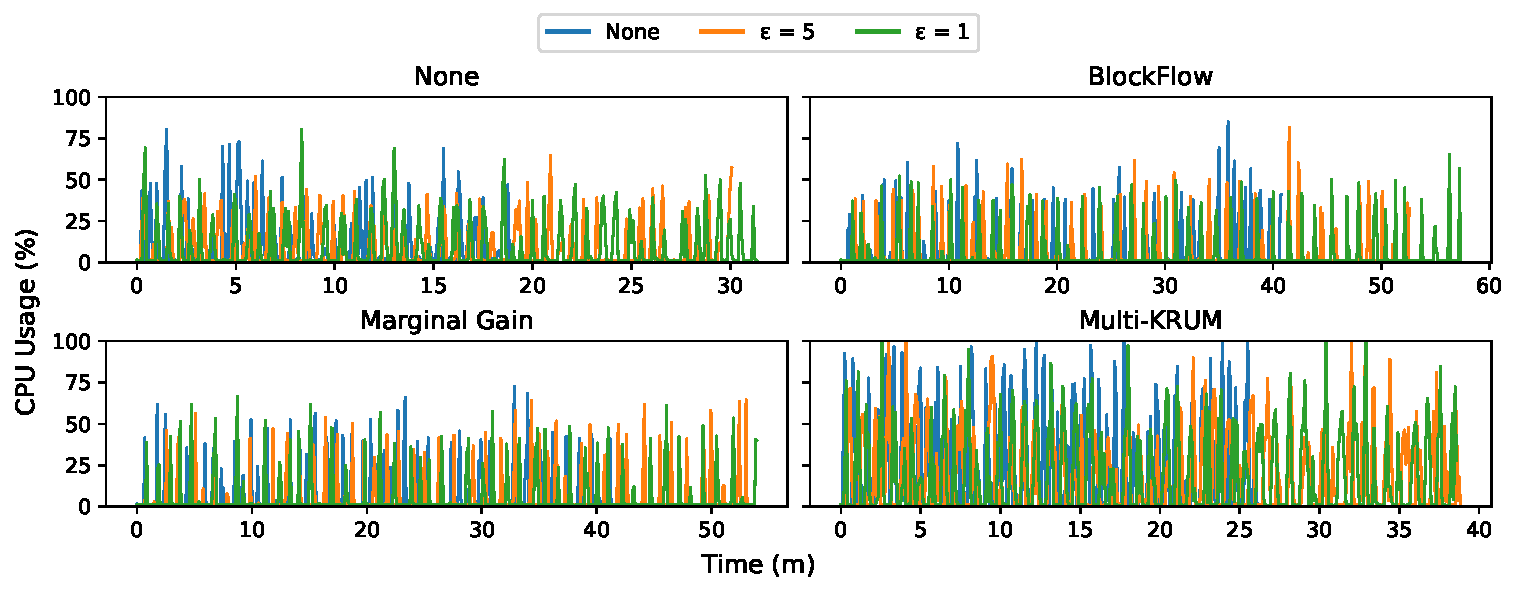
\includegraphics[width=\textwidth]{graphics/privacy/cpu_server.pdf}
    \caption{Server Process CPU Usage Per Privacy Degree}
    \label{fig:cpu_privacy_servers}
\end{figure}

\vfill

\begin{figure}[!h]
    \centering
    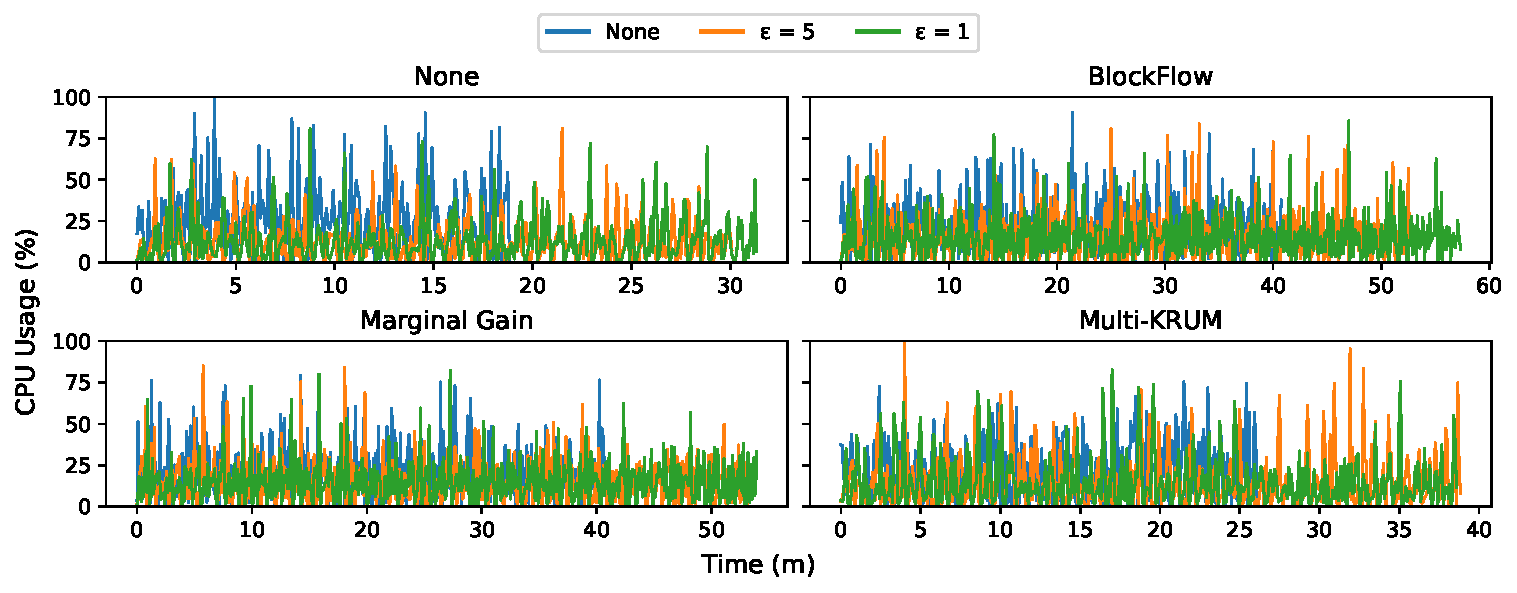
\includegraphics[width=\textwidth]{graphics/privacy/cpu_miner.pdf}
    \caption{Blockchain Process CPU Usage Per Privacy Degree}
    \label{fig:cpu_privacy_miners}
\end{figure}
